\newcount\draft\draft=0
\newcount\cameraready\cameraready=0

% This version uses the latex2e styles, not the very ancient 2.09 stuff.
\documentclass[letterpaper,twocolumn,10pt]{article}
\usepackage{usenix,epsfig,endnotes}
\usepackage[T1]{fontenc}
\usepackage{soul} % for using hl{}
\usepackage{graphicx,epsfig,sped,times,wide}
\usepackage{algorithm,url}
\usepackage{clrscode}
\usepackage[noeka]{mathrmletter}
%\usepackage{subfigure}
\usepackage{subfig}
\usepackage{soul}
\usepackage{url}
\usepackage{epstopdf}
\usepackage{ulem}
\usepackage{comment}
\usepackage{amsmath}
\renewcommand{\em}{\normalem}

\usepackage{multirow}
\usepackage[noend]{algorithmic}
%\usepackage{natbib}
\usepackage[bookmarks, colorlinks=false, plainpages = false]{hyperref}
%\usepackage[bookmarksnumbered,colorlinks,backref, bookmarks, breaklinks]{hyperref}
%\urlstyle{rm} %so it doesn’t use a typewriter font for url’s.

\epstopdfsetup{outdir=./}

\ifnum\draft=0
% \input{revision}
% \usepackage{drafthead}
\fi

%Begin boilerplate
\newfont{\mycrnotice}{ptmr8t at 7pt}
\newfont{\myconfname}{ptmri8t at 7pt}
\let\crnotice\mycrnotice%
\let\confname\myconfname%
%End boilerplate

\newcommand{\vitag} {ViTag}
\newcommand{\reader} {ViReader}
\newcommand{\retro} {Retro-VLC}

\newenvironment{Itemize}%
{\begin{itemize}%
\setlength{\itemsep}{0pt}%
\setlength{\topsep}{0pt}%
\setlength{\partopsep}{0pt}%
\setlength{\parskip}{0pt}}%
{\end{itemize}}
\setlength{\leftmargini}{0pt}%

\newenvironment{Enumerate}%
{\begin{enumerate}%
\setlength{\itemsep}{0pt}%
\setlength{\topsep}{0pt}%
\setlength{\partopsep}{0pt}%
\setlength{\parskip}{0pt}}%
{\end{enumerate}}
\setlength{\leftmargini}{1.25em}%

%----special-caption-magic--------%

\makeatletter
  \newcommand\figcaption{\def\@captype{figure}\caption}
  \newcommand\tabcaption{\def\@captype{table}\caption}
\makeatother

%---- Theorem Environment ----------------%
\newtheorem{theorem}{Theorem}[section]
\newtheorem{lemma}[theorem]{Lemma}
\newtheorem{proposition}[theorem]{Proposition}
\newtheorem{corollary}[theorem]{Corollary}

\newenvironment{xproof}[1][Proof]{\begin{trivlist}
\item[\hskip \labelsep {\bfseries #1}]}{\end{trivlist}}
\newenvironment{xdefinition}[1][Definition]{\begin{trivlist}
\item[\hskip \labelsep {\bfseries #1}]}{\end{trivlist}}
\newenvironment{xexample}[1][Example]{\begin{trivlist}
\item[\hskip \labelsep {\bfseries #1}]}{\end{trivlist}}
\newenvironment{xremark}[1][Remark]{\begin{trivlist}
\item[\hskip \labelsep {\bfseries #1}]}{\end{trivlist}}
%\newenvironment{proof}[1][Proof]{\begin{trivlist}
%\item[\hskip \labelsep {\bfseries #1}]}{\end{trivlist}}
\newenvironment{definition}[1][Definition]{\begin{trivlist}
\item[\hskip \labelsep {\bfseries #1}]}{\end{trivlist}}
\newenvironment{example}[1][Example]{\begin{trivlist}
\item[\hskip \labelsep {\bfseries #1}]}{\end{trivlist}}
\newenvironment{remark}[1][Remark]{\begin{trivlist}
\item[\hskip \labelsep {\bfseries #1}]}{\end{trivlist}}

\newcommand{\xqed}{\nobreak \ifvmode \relax \else
      \ifdim\lastskip<1.5em \hskip-\lastskip
      \hskip1.5em plus0em minus0.5em \fi \nobreak
      \vrule height0.75em width0.5em depth0.25em\fi}

\newcommand{\xref}[1]{\S\ref{#1}}
\newcommand{\pxref}[1]{(\S\ref{#1})}
\newcommand{\algref}[1]{Algorithm~\ref{#1}}
\newcommand{\figref}[1]{Fig.~\ref{#1}}
\newcommand{\para}[1]{\vskip 0.06in\noindent {\bf #1} }


% peanut gallery comments
%
%
% NOTE: Comment *in* the line below if you want a draft with no red comments.
% NOTE: Doing so may replace some of the red comments with 
%       extra spaces or newlines.
%\def\noeditingmarks{}
%
\newcommand{\textred}[1]{\textcolor{red}{#1}}
\ifx\noeditingmarks\undefined
   \newcommand{\pgwrapper}[2]{\textred{#1: #2}}
\else
   \newcommand{\pgwrapper}[2]{}
\fi
\newcommand{\sg}[1]{\pgwrapper{SG}{#1}}
\newcommand{\hh}[1]{\pgwrapper{HH}{#1}}
\newcommand{\dk}[1]{\pgwrapper{DK}{#1}}
% end peanut gallery comments

\usepackage{xxx} % somewhat nicer peanut-gallery comments: \xxx[whom]{comment}

%\renewcommand{\dbltopfraction}{0.1}
\frenchspacing

% margins
\setlength{\topmargin}{-0.2in} 
\setlength{\textheight}{9.3in}
\setlength{\evensidemargin}{-.2in}
\setlength{\textwidth}{6.99in}
\setlength{\columnsep}{.33in}
%\setlength{\parindent}{.2in}
%\renewcommand{\topfraction}{1.00}
%\renewcommand{\textfraction}{0.20}

% section styles - ACM bastards
\makeatletter

\global\def\section{\@startsection {section}{1}{\z@}%
                                   {2ex \@plus 1ex \@minus .1ex}%
                                   {1ex \@plus.2ex}%
                                   {\normalfont\bfseries\scshape\fontsize{11}{13}\selectfont}}
\global\def\subsection{\@startsection{subsection}{2}{\z@}%
                                     {2ex\@plus 1ex \@minus .1ex}%
                                     {1ex \@plus .2ex}%
                                     {\normalfont\bfseries\fontsize{10}{12}\selectfont}}
%%\global\def\subsubsection{\@startsection{subsubsection}{3}{\z@}%
%%                                     {2ex\@plus 1ex \@minus .1ex}%
%%                                     {1ex \@plus .2ex}%
%%                                     {\normalfont\itshape\fontsize{10}{12}\selectfont}}

% \def\@maketitle{\newpage
%  \null
%  \setbox\@acmtitlebox\vbox{%
% \baselineskip 20pt
% \vskip 2em                   % Vertical space above title.
%    \begin{center}
%     {\ttlfnt \@title\par}       % Title set in 18pt Helvetica (Arial) bold size.
%     \vskip 1.5em                % Vertical space after title.
% %This should be the subtitle.
% {\subttlfnt \the\subtitletext\par}\vskip 1.25em%\fi
%     {\baselineskip 16pt\aufnt   % each author set in \12 pt Arial, in a
%      \lineskip .5em             % tabular environment
%     \begin{tabular}[t]{c}\hspace{-.15cm}\@author
% %     \begin{tabular}[t]{p{\auwidth}}\centering\@author
%      \end{tabular}\par}
%     \vskip 1.5em               % Vertical space after author.
%    \end{center}}
%  \dimen0=\ht\@acmtitlebox
%  %\advance\dimen0 by -12.75pc\relax % Increased space for title box -- KBT
%  \advance\dimen0 by -10pc\relax % Increased space for title box -- KBT
%  \unvbox\@acmtitlebox
%  \ifdim\dimen0<0.0pt\relax\vskip-\dimen0\fi}

\def\sharedaffiliation{%
\end{tabular}
\begin{tabular}{c}}










\begin{document}

%VINFIX for overflow
\font\ttlfnt=phvb8t at 17pt

\title{\retro: Low-Power Duplex Visible Light Communication}
%%Rethinking Communication Primitives for Backscatter Devices

\newcommand{\supsym}[1]{\raisebox{6pt}{{\footnotesize #1}}}


\widowpenalty = 10000


\author{
%Working Draft\\
XXX\\
}


%don't want date printed
\date{}
\maketitle

\begin{sloppypar}

\begin{abstract}
The new generation of LED-based illuminating infrastructures has enabled a ``dual-paradigm" where LEDs are used for both illumination and communication purposes. The ubiquity of lighting makes visible light communication (VLC) well suited for communication with mobile devices and sensor nodes in indoor environment.
Existing research on VLC has primarily been focused on advancing the performance of one-way communication. %We argue that it is essential to have bi-directional communication capability and simple combination of two one-way VLC is ill-suited for the communication between the lighting infrastructure and a mobile device.
In this paper, we present \retro, a low-power duplex VLC system that enables a mobile device to perform bi-directional communication with the illuminating LEDs over the same light carrier. The design features a retro-reflector fabric that backscatters light, an LCD shutter that modulates information bits on the backscattered light carrier, and several low-power optimization techniques. We have prototyped the \fyi{reader} system and made a few battery-free tag devices. \fyi{Experimental results show that the tag can achieve a $10kbps$ downlink speed and $0.5kbps$ uplink speed over a distance of $2.4m$. We also outline several potential applications of the proposed \retro\ system. } 

%The visible light has been used as a wireless carrier for data communication. Existing designs of Visible Light Communication (VLC) systems, however, consume significant power and only achieve one-directional communications where the mobile device is unable to transmit data to the light bulb on the same band, and hence cannot be applied to low complexity, power-constrained mobile devices or in an interactive manner without occupying extra bandwidth, extremely limiting the use of VLC in mobile and networked settings. This paper makes two main contributions: (1) we introduce the first duplex VLC system design that operates on credit card-sized battery-free devices, and (2) we introduce a communication primitive applicable to secure Radio-Frequency IDentification (RFID) systems acting against side sniffers. 
 %, and (3) we introduce a novel algorithm to detect weak and distorted signals out of strong interferences on the same spectrum that makes the system scalable
% We build a hardware prototype of the above design that can be powered solely using harvested energy from the Light-Emitting Diode (LED). The results show that our design provides benefits for VLC systems and RFID systems: it enables battery-free devices to communicate with LEDs at data rates of $10kbps$ on the downlink and $1kbps$ on the uplink and over a maximum distance of $2.2m$; it limits the uplink signal exposure area within a spindle-shaped area whose radius is less than $0.2m$. We believe that this paper represents a substantial leap in the capability and scalability of VLC systems towards previously infeasible battery-free, duplex, always and anywhere-available and secure ubiquitous communication applications.
\end{abstract}

% A category with the (minimum) three required fields

% one file per section means fewer conflicts to resolve during multiparty
% editing

\section{Introduction}

\begin{figure}[!t]
\vskip -0.03in
  \centering
      {
        \epsfig{file=../illustrations/sysdiagram.eps, width=0.6\columnwidth}
      }
\caption{{\bf Our \vitag\ Prototype} \hl{integrates both mmm in a single design. It can operate using both RFID and TV transmissions}.}
\label{fig:tag}
\vskip -0.05in
\end{figure}

%\p{VLC is promising direction}
Nowadays, LEDs have been prevalently deployed for illumination purpose for its advantageous properties such as high energy efficiency, long lifetime, environment friendliness, to name a few. Being semiconductor devices, LEDs also possess another feature, i.e.\, it can be turned on and off instantaneously. This effectively turns LED lights into a carrier and gives rise to a new ''dual-paradigm'' -- illumination and communication -- of LED lighting. Thanks to the ubiquity of lighting infrastructure, visible light communication (VLC) has thus attracted lots of research interest~\cite{fundamental1, fundamental2, standard}. A standard (IEEE 802.15.7) has been established recently~\cite{standard} to ensure inter-operation among device manufacturers. Some practical systems such as ByteLight~\cite{ble0} have debuted the exploitation of LED lighting infrastructures for both communication and localization~\cite{location1,location2}. 

%\p{existing solution does not meet two-way communication need}
Existing work has primarily focused on exploring or improving the one-way link from the LEDs to the mobile ends, i.e.\, from the LEDs to the receiving small computing devices. Indeed, significant advances have been made, e.g.\, VLC systems today can achieve bit rates up to $~10Mbps$ from an LED transmitter to a receiver over a distance of $~10km$~\cite{expensive,expensive2,retro1,retro2}. However, despite these promising results, it solves only half of an actual communication system where two-way communications are essential. In response, in ByteLight and many other smart light system with remote control, a BlueTooth Low Energy link is typically leveraged as the uplink to send information or control messages from a mobile device to the light. 

%\p{The need of low-power solution, not affordable to use LED at mobile device.}
The dual-paradigm nature of LED lighting, with illumination as the primary goal, naturally leads to an asymmetric communication setting. The transmitters, i.e., LEDs, are externally powered and can emit strong signals, whereas the receivers are typically small computing devices such as mobile phones and even weaker sensors. Applying the LED-photodiode link straightforwardly from a mobile device or sensor node to the lighting LED is not affordable. A typical VLC system consists of an LED, a photodiode and intermediate optical components (e.g., lenses). To achieve high speeds as reported in literatures~\cite{expensive,expensive2,flawedsys3,flawedsys4}, special and expensive hardware pieces such as multiple quantum well electro-absorption modulators and lasers have to be used~\cite{expensive}; They consume orders of magnitude more power than is available on credit-card-sized devices that harvest energy from LED lights~\cite{solarsheet}. In this light, we focus on using ordinary lighting LEDs whose primary goal is illumination. In such a setting, the LED flickering rate is relatively low. For instance, we measured that the rising and falling frequency of an ordinary commodity LED bulb is at most $1MHz$.

% \fye{
% This ubiquity opens a door for the LEDs to communicate with small computing devices with the emitted lights. The last few years have seen significant advances in VLC systems --- VLC systems today can achieve bit rates up to \hl{ss Mbps} from an LED transmitter to a receiver over a distance of \hl{ss}~\cite{flawedsys1,flawedsys2,flawedsys3,flawedsys4}. Researchers have also demonstrated the VLC capability of providing location services~\cite{location1,location2}. These impressive capabilities are made possible by systems that encode and modulate the light emitted by the LED. However, all these systems, on one hand, either support one-directional communications only from the LED to the device, or require the mobile device to have additional LED~\cite{led2led1}, Bluetooth~\cite{ble1} or other facilities~\cite{retro1,retro2} to transmit the uplink data; On the other hand, achieving such high data rate requires complicated modulation schemes and power-expensive analog-to-digital converters (ADCs) that consume power on the order of \hl{10mW}~\cite{flawedsys1}, alongside the power needed for driving those facilities; this is orders of magnitude more power than is available on credit card-sized devices that harvest power from ambient light sources~\cite{solarsheet}.
% }

% \p{our goal -- very low power bi-directional VLC, low enough to be affordable by harvesting energy from the LED light. Compared with RFID, it has more favorable security features. }
In this paper, we ask if it is possible to achieve very low power bi-directional VLC where the mobile end is affordable solely by harvesting energy from the LED light. Such a system would not only work at any location with LEDs at any time, but would also remedy the security flaws typically faced by existing RFID systems, where the uplink transmission tends to be exposed to a wide area of space, leaving chances for sniffers and attackers to temper the system. Thus, a positive answer would enable ubiquitous communication with access to existing network infrastructures at unprecedented spacial and temporal scales with user security preservation. 

%\p{core idea: leverage the retro-reflector to avoid the need of generating high power visible light; use LCD to modulate the reflected lights. }
Our core idea is as follows. To avoid generating power-expensive visible lights on the mobile end, we use a toggling \textit{Liquid-Crystal Display (LCD)} to modulate a \textit{retro-reflector} that directionally bounces the incoming light back to the LED, which forms a low-power uplink.   

%\p{challenges in achieving the low-power goal: 1) energy consumption at the receiver side; 2) LCD energy consumption at high toggling frequency at the transmitter side; 3) weak signal detection; 4) clock-drift handling at the LED side, without explicit synchronization between transmitter and receiver. }
Designing such a system, however, is challenging for the following reasons:
\begin{Itemize}
\item Demodulating and decoding the high throughput LED-transmitted data is power consuming. 
\item Transmitting with the LCD at a high toggling frequency consumes even more power than the receiver.
\item The LED has to detect retro-reflected signals 3 orders of magnitude weaker than its interfering transmissions.
\item The LED must handle clock offsets on the mobile end that uses a low-cost clock with low oscillating frequency.   
\end{Itemize}
%as (1) generating light waves and modulating them typically require much more power than can be harvested from ambient light sources by a small device (see~\ref{sec:app}), and moreover, (2) detecting signals sent by the device at the LED receiver against interferences is hard. In this paper, we introduce \vitag, a VLC system that provides duplex communication capabilities on battery-free devices only using visible light carriers. To address the challenge of detecting signals against interferences on the LED receiver, \vitag\ uses a novel algorithm specifically designed for the LCD-modulated signals. Instead of generating signals, \vitag\ addresses the power constraint challenge by backscattering the incoming light waves using retro-reflectors and modulating using Liquid-Crystal Displays (LCDs). This helps the backscattered signal focus at the receiver on the LED, and avoids generating signals on \vitag. In addition, \vitag\ recycles the LCD modulation energy with an energy reuse module, further optimizing the mobile device size to the size of a regular credit card. Finally, there are a set of other techniques behind the \vitag\ design that make it feasible in real-world illumination system deployment, which we will describe in later sections.

%\p{our design: principles -- 1) use analog components as much as possible (to avoid ADC) and complicated digital signal processing; 2) circuit design to recycle energy for lcd; 3) differential amplifier design? 4) windowed multi-symbol match filter}
To address these challenges, we apply the following design principles:
% \begin{Itemize}
% \item Use differential tunning analog components and avoid complicated digital signal processing on the mobile end to conserve energy while achieving comparable accuracy to when ADCs are used. 
% \item Recycle energy spared by the LCD at every toggle.
% \item Design amplifiers that work at an almost cut-off state to further reduce energy consumption.
% \item Design a sliding-window multi-symbol match filter algorithm to remedy clock drifts and LCD-caused signal distortions.
% \end{Itemize}

\begin{Itemize}
\item Use analog components over digital ones while achieving comparable accuracy.
\item Recycle LCD energy. 
\item Design energy efficient amplifiers.
\item Design algorithms to decode signals that suffer from severe clock offsets caused by low-cost mobile end.
\end{Itemize}

%\textbf{\retro.} To understand our \vitag\ design on battery-free ID card-sized tags, consider an LCD whose emitted light can be manipulated by an additional small circuit inside the light bulb. This circuit embeds information in the light and modulates it, while keeping the brightness of the light the same without any flickering. On the \vitag\ side, a light sensor captures the light signal that conveys information from the LED. To conserve energy, \vitag\ only uses analog components to demodulate the signal without an ADC. Upon detecting data, a low-power micro-controller on \vitag\ is waked up for uplink data transmission. It drives up the LCD to flicker, therefore sending data back to the LED by backscattering the light with a retro-reflector behind the LCD. This uplink data can be captured by a light sensor placed on the LED, along with interferences caused by downlink transmission, nearby human and object movements, household electricity fluctuations, and so on. A specifically designed receiver associated with the LED then performs the time recovery and demodulates the signal. To get a network of \vitag\/s and LEDs into play, we design a Media Access Control (MAC) protocol to mediate the communications in LEDs' illumination range. 

%\p{We demonstrated the design with a batter-free ViTag by harvesting LED light energy. We explore the tradeoff between the solar panel area and retro-reflector area to achieve a maximum working range for a typical lux level. }\todo{This suggests that the optimal value be a function of the solar cell efficiency and the reflecting concentration ratio.}
We demonstrated the design with a battery-free credit-card-sized \textbf{\vitag}, as shown in Fig.~\ref{fig:tag}, that harvests energy of off-the-shelf LED lights. We also explored the tradeoff between the solar panel area and the retro-reflector area for achieving a maximum working range at a typical $lux$ level. 
%To show the feasibility of our ideas, we have built a hardware prototype, shown in Fig.~\ref{fig:tag}, that is approximately the size of a credit card. Our prototype includes multiple off-the-shelf LEDs emitting white lights, LED transmitters each stuffed inside an LED, LED receiver PCBs and \vitag\ PCBs. LEDs and \vitag\/s are equipped with a micro-controller, respectively. Our prototype also includes a solar cell of size \hl{ss $\times$ ss} on \vitag.

We evaluate our system in locations where illuminating LEDs are typically deployed, including offices and evening streets. We also evaluate in dark chambers as the baseline. We measure the maximum communication range between the LED and the \vitag\ in varying $lux$, \vitag\ orientation, angle of incidence, solar panel area and retro-reflector area settings. Our experiments show that our \hl{ss $\times$ ss} \vitag\ prototype can achieve a bit rate of \hl{10kbps} on the downlink and \hl{1kbps} on the uplink at distances of up to \hl{2.2m} in dark chambers, \hl{2.0m} on sidewalks in the evening, and \hl{1.5 m} in offices, under the power budget of \hl{400 $\mu W$}. We also evaluate the area in which \vitag\ uplink transmission can be sniffed or tempered. Experiments show \vitag's uplink transmission cannot be detected over the radius of \hl{m}, and malicious readers cannot detect uplink transmissions when \hl{m} away from \vitag\/s.

%\p{contributions: 1) propose the use of retro-reflector for practical two-way VLC; 2) address various challenges; 3) build and evaluate a real prototype system.}
\vskip 0.05in\noindent{\bf Contributions:} We make the following contributions:
\begin{Itemize}
\item We propose the first practical bi-directional VLC primitive that works for small battery-free devices using retro-reflectors and LCDs and ordinary white LEDs.
\item We address various challenges by designing energy-efficient components on the \vitag\ and an unsynchronized decoding scheme on the LED.
\item Finally, we build and evaluate a prototype system which shows all of the above.
\end{Itemize}
%\begin{Itemize}
%\item We present \vitag, the first visible light duplex communication system design that operates on battery-free devices while retaining a small size for them.
%\item We develop a secure communication primitive applicable to RFID systems that acts against side sniffers and malicious transmitters.
%\item Finally, we present designs and build a prototype which shows how all of the above, from \vitag, modified LEDs, through to the network stack, can be implemented on credit-card sized battery-free devices at a low cost.
%\end{Itemize}



\section{Related Work}


Our work is related to prior work in VLC systems and backscatter communication systems:

\vskip 0.05in\noindent{\bf (a) VLC Systems:} 
%Because LEDs are ubiquitously deployed, there have been efforts to turn them into communication-capable devices. 
Recently, there have been many efforts exploring communication mediums wherein visible lights carry information. 
These \fyi{work}, however, either deal with only one-way communication without an uplink~\cite{flawedsys1,flawedsys2,flawedsys3,flawedsys4}, or go in a two-way fashion with both sides supplied by battery~\cite{led2led1,led2led2,led2led3}, which limit real-world practicality. Specifically, LED-to-phone systems~\cite{location1,location2,location3} only support downlink transmissions, targeted at phone localization. LED-to-LED systems~\cite{led2led4,led2led5} consider visible light networks, where each end is not meant to be mobile, and is not battery-free. 
%LED-Bluetooth systems~\cite{ble0} provide the uplink capability using Bluetooth, but the system occupies an additional band to provide such uplink capability, and is not battery free. 
By contrast, our work augments the existing systems with an additional uplink channel from the mobile device to the LED on the same band as the downlink, with an emphasis on the low power design and system robustness. %instead of boosting data rate.
%while eliminating the need for battery supply for the mobile device.

%\p{RFID, then ambientscatter. Amb scatter is for communication between devices, not to communication based to the energy source. Be our future work. }
\vskip 0.05in\noindent{\bf (b) Backscatter Systems:} 
Backscattering is a way to provide transmission capability for extremely low-power devices, substituting the need for devices actively generating signals. The technique has been primarily used by RFID tags~\cite{rfid1,rfid2}. Recently, Wi-Fi ~\cite{abc3} and TV-based ~\cite{abc1,abc2} systems started employing and advancing this technique. 


Our \retro\ system also achieves low-energy design using backscattering and further shares design principles with \cite{abc1,abc2, abc3}, that is, using analog components on the energy-constrained end. The major differences lie in the fact that we are dealing with visible light using a retro-reflector, whereas the ambient backscatter systems are backscattering radio waves. On the tag side, we use a light sensor to receive and a retro-reflector to send (by reflection) information, which is also different from the shared antenna and RF front-end in other backscattering systems. In comparison, we can easily achieve full-duplex while other systems are essentially half-duplex and require intensive tricks and significant overhead to achieve full-duplex \cite{fullduplex1,fullduplex2,fullduplex3}. 

%Due to the ubiquity of light infrastructure, our system can be widely applied, especially in indoor environments, whereas TV signal backscattering~\cite{abc1,abc2} systems are limited to areas close to TV tower, and Wi-Fi backscattering~\cite{abc3} further limits the communication range to be very close to the AP and can only work intermittently due to Wi-Fi signal's bursty nature. The TV-based backscattering systems aims at enabling communication among devices, instead of communication back to the infrastructure. 

%RFID systems~\cite{rfid1,rfid2} typically include a passive tag, too. However, first, RFID systems need a second-order modulation on the tag to eliminate base band noise, while \vitag's uplink does not have any second-order modulation, relying on the \reader\ who conducts demodulation and decoding algorithms to extract useful information. Second, RFID readers are not ubiquitous as LEDs, and readers are not readily networked like LEDs~\cite{flawedsys1}. Finally, in terms of capability, in comparison with NFC RFID systems~\cite{iso1}, visible lights can transmit farther in the line-of-sight scenario; as for vicinity RFID systems~\cite{iso2}, visible lights transmit more stably, in the sense that a transmission is not as easily distorted by surrounding object movements.

%TV signal backscattering~\cite{abc1,abc2} works at a band around $539MHz$, leveraging the existing TV signals to power up small devices to do communications. However, the locations at which these systems can work are extremely limited. In typically indoor environments, TV signals cannot be detected everywhere~\cite{abc2}. Plus, there isn't any uplink from these devices to TV towers.

%Wi-Fi backscattering~\cite{abc3} is an alternative that provides both downlink and uplink transmissions for battery-free devices around Wi-Fi routers. However, due to Wi-Fi signals' bursty nature, the communication is not really available all the time; when there is no ongoing Wi-Fi packets, neither can enough radio energy be harvested nor are there signals to be modulated by devices.

%Finally, in general, these backscattering systems tend to expose their transmissions to a wide area, because of the scattering nature. This potentially gives side readers a chance to overhear the information being transmitted~\cite{abc1,abc2,abc3}. By contrast, \vitag relies on visible light communication, which implies eavesdroppers are easily discernible. The use of retro-reflectors further retains the uplink transmission along the tag-reader path. As a result, our system comes with a good security property inherently while systems on other bands have to enhance their security with extra efforts~\cite{eavesdrop1,eavesdrop2}.

In addition, because of the backscattering nature, these wireless systems tend to expose their transmissions to a wide surrounding area, leaving a good chance for side readers to overhear the information being transmitted~\cite{abc1,abc2,abc3}. By contrast, \vitag relies on visible light communication, which implies that eavesdroppers are easily discernible. The use of retro-reflectors further constraints the uplink transmission to stick along the tag-reader path. As a result, our system \vitag comes with a good security property inherently, while other systems have to enhance their security with extra efforts~\cite{eavesdrop1,eavesdrop2}.


% \vskip 0.05in\noindent{\bf (c) Duplex Systems:} Previously, it is either the case that systems built on visible light bands are non-duplex~\cite{flawedsys1}, or that duplex systems are not both operating at visible light frequencies~\cite{ble1,ble2,ble3,ble4}. Moreover, radio systems that achieve the full-duplex feature require intensive interference cancellation and noise filtering tricks that consume a huge amount of energy on the backscatter side, of which FFT and dynamic adaption are the most energy demanding components~\cite{fullduplex1,fullduplex2,fullduplex3}. In the \vitag\ design, we avoid heavy energy consumption by focusing the uplink energy better at the LED receiver. In lieu of the use of complex digital signal processing components by current designs on the back-scatterer end~\cite{fullduplex4,fullduplex5}, the careful design of an error-restricting time recovery algorithm in our design helps hugely remove the interference caused by reflection of the signals transmitted by \reader\ itself, adapting the systems to almost all kinds of lightening conditions. We also design an energy collection module that retrieves the residual energy in the course of LCD discharge, such that the tag size can be minimized while retaining the battery-free feature.

% At TV frequencies, a recent work on full-duplex backscatter system~\cite{abc5} uses different frequencies for the uplink and downlink, respectively, on the signal envelope. However, it lacks scalability and is not resource-efficient. \vitag\, as mentioned earlier, has focused uplink transmissions and does not differentiate the carrier frequency between the uplink and downlink, easily scalable to a network with multiple LEDs and mobile devices. 
\section{Preliminaries}
\label{sec:background}

\begin{figure*}[!t]
\vskip -0.1in
\centering
{\footnotesize
\begin{tabular}{cccc}
\epsfig{file=../illustrations/mrr1.eps, width=0.5\columnwidth} &
\epsfig{file=../illustrations/mrr2.eps, width=0.5\columnwidth} & 
\epsfig{file=../illustrations/mrr3.eps, width=0.5\columnwidth} & 
\epsfig{file=../illustrations/mrr4.eps, width=0.5\columnwidth} \\
{(a) Same Direction} & {(b) Different Directions} & {(c) With LCD on} & {(d) Retro-reflector Principle}\\
\end{tabular}
}
\vskip -0.1in
\caption{\footnotesize{\bf Illustration of the Retro-reflector.} Blah Blah.}
\label{fig:retrolcd}
\vspace{-1em}
\end{figure*}



In this section, we introduce a few concepts which are used throughout the paper. 

%In principle, \vitag\ is a general technique that can leverage visible light signals to do full-stack secure communications between an array of powered sources and battery-free backscatter devices. In this paper, we demonstrate this feasibility with an RFID-based application, and show that it is better than the existing RFID technology in several critical aspects. 

\paragraph{Visible Light Communication} 
Visible lights are electromagnetic waves that span frequencies roughly from $400$ to $800 THz$. Commonly, white LEDs are used for illumination. The instantaneous On/Off feature turns LEDs into effective transmitters for visible light communication (VLC). Specifically, information bits can be embedded on the light by modulating the on/off state of the LED with on-off keying (OOK) or variable pulse-position modulation (VPPM) \cite{standard}. To receive such signals, while in some cases a cell phone camera or a digital camera will be sufficient \hl{need citations, ipsn14 and mobicom14}, photodiodes are generally used, because phone cameras can only achieve around 0.25MHz sampling rate~\cite{camera1} (in other words, low data rate), whereas photodiodes have generally higher bandwidth up to 0.5GHz~\cite{pdsheet}. Moreover, compared with a phone camera, the SNR of the photodiode is orders of magnitude higher at the same distance \hl{ipsn14}. 

%A typical way to generate white lights is to use a phosphor material to convert monochromatic lights from blue or ultraviolet to broad-band white lights, where the color of the monochromatic light depends on the band gap energy of the materials forming the p-n junction in the LED. 

%Visible lights bring safety advantages over communication waves of other common frequencies, because human eyes are much more sensitive to the strength of visible lights than the invisible TV, Wi-FI and RFID transmissions. With the LED dimming support~\cite{dimming}, a person can turn down the light if she feels of a too high brightness. In addition, radios waves at some certain frequencies are likely to hard human organs, especially to pregnant women and kids~\cite{rfidharm}, while the visible light are not.

%There are two primary ways of producing white LEDs. One is to use individual LEDs that emit three primary colors --- red, green, and blue --- and then mix all the colors to form white light~\cite{ledprin1}. The other is to use a phosphor material to convert monochromatic light from a blue or UV LED to broad-spectrum white light, much in the same way a fluorescent light bulb works~\cite{ledprin2}. In general, the wavelength of the light emitted, and thus its color, depends on the band gap energy of the materials forming the p-n junction. In materials used for LEDs, the electrons and holes recombine by a radiative transition, which produces optical emission, because there are direct band gap with energies corresponding to near-infrared, visible, or near-ultraviolet light. 



\paragraph{Retro-reflector} 
Retro-reflector is a device or surface that operate by returning light back to the light source along the same light direction with a minimum of scattering \hl{cite the wikipage}. Retro-reflectors are widely used on road signs, bicycles, and clothing for road safety. From a microscopic view, a retro-reflector is composed of cells, each of which is a corner cube as shown in \hl{Fig.xx}. When a light beam hits one of the cells, the light is turned around via two adjacent reflections. 

Modulating retro-reflector (MRR) \hl{cite the wikipage} is a system typically consisting of a retro-reflector and a modulator for optical communications. The MRR operates as a passive sources which transmits bits by varying the intensity of the reflected light beam. MRR is widely used in free space communication where the other side is a laser. Existing MRR \hl{cite some papers} is usually with large size, and modulation is commonly achieved with a high-end electroabsorption modulator altering the absorption spectrum by applying an electric field. Consequently, such setting is ill-suited for our scenarios which require a low-cost solution.

\p{Need double check. It is really hard to understand the existing MRR solutions. Cannot find much material.}

 
\paragraph{Liquid-crystal display (LCD)}
LCD is a type of display widely used in portable devices like digital watches and phones. LCDs do not emit light directly; Rather, they use the light properties of liquid crystals that are controlled by the voltage added on them. When the LCD is on, the incoming light is able to pass the LCD and hit the retro-reflector; When the LCD is off, the incoming light is rejected by the LCD. Therefore, LCDs can be used as modulators for MRRs. However, one disadvantage of LCDs are their low refresh rate, e.g., 60 or 75 Hz, which is too low for data communication. Fortunately, we find \textit{LCD shutters} with much higher refresh rate (up to 1KHz \hl{cite}). Fig.~\ref{fig:retrolcd} shows the basic principle of a retro-reflector with an LCD coverage.


\section{Our Design Principle}

Our goal is to design primitives that enhance visible light communication capabilities on battery-free devices while preserving user privacy and security of both the transmitters and the receivers, with the omnipresence of readily available LEDs that serve as the lightening devices. The key challenge in achieving these is two-fold. First, devices running at visible light bands are power-intensive because of the broad bandwidth these bands can provide. Second, the noise caused by ambient signals on the visible light spectrum and the interference triggered by the the data transmitted by the system itself stays in the same band as what the receiver expects to receive at. To address these challenges, we use the following guiding principles: we use as many analog components and recycle as much energy as possible on the tag to enable the tag to transmit to the reader with a decent data rate. Also, we diminish the scattering area as much as possible by making use of directional backscattering materials of small Field of View (FoV). Such approaches, as we show in the rest of the paper, can provide an order of magnitude reduction in the power consumption of these communication primitives and in the scattering area of the signals on the backscattering channel.

In the rest of this paper, we describe \vitag, our battery-free tag and show how it can enable backscatter communications with no battery and with a higher energy efficiency with respect to communication range than tags with LEDs on. We then describe \reader, our system that can be easily integrated onto commercial LED lights for transmitting data at no discernible flickers with dimming support and receiving with \hl{hhh dB} signal-to-interference-plus-noise-ratio (SINR). Finally, we show that our designs can be used to enable concurrent transmissions in a network of battery-free devices without the need for synchronization.
\input{\vitag}
%\input{\reader}
\section{Discussions}

\paragraph{Full Duplex vs Half Duplex}
Unlike radio backscattering systems where achieving full duplex is extremely challenging due to shared antenna and RF front-end, full duplexing is natural to \retro. This attributes to the fact that separate components are responsible for emitting (LED/retro-reflector) and receiving (photodiode) light. The only difference is that, in full duplexing, the reflected light contains downlink signals whereas in half duplexing, the reflected light is the pure carrier. The different reflected carriers have no impact on the decoding of uplink, due to LPF at the reader frontend.  Full duplexing also incurs extra power consumption as both the receiving and transmitting logics are active and the MCU will be kept at a high working frequency.%, whereas in half duplexing, the MCU will work very low frequency during uplink transmission. 
 
%Our design support both working modes. The major difference is the modulation of the uplink is performed on a pure carrier for the half-duplex mode whereas it will be on the infomation-carrying carrier for the full-duplex mode. In this particular design, as the carrier frequence is much higher (1MHz) and the Manchester coding we used, the basic frequency components of the information-carrying is far apart from the basic frequency components that we used to carry information in the uplink. In addition, in full duplex mode, we may reuse the higher and more accurate clock of the MCU instead of using a RC oscillator. Therefore, the decoding on the ViReader side can be more accurate. The only penalty is that full-duplex will consumes more energy at the ViTag side as both the receiving and transmitting modules are active at the same time, whereas in half-duplex model, they are alternatively active.

%\paragraph{Active Emitting v.s. Backscattering.} 
%We note that it is also possible to use LEDs on \vitag\ to deliver uplink data transmission using a battery-free design\footnote{This could be achieved by doing smart duty-cycling and adding a capacitor next to the solar cell array to provide the $1mA$ peak current supply for the LED.} in place of the use of retro-reflectors and LCDs. We show, however, that 
%\begin{lemma}
%In general cases\footnote{To form a fair comparison, we set the \reader\ LEDs, the light sensors attached to \reader, \vitag-\reader\ distances, working bit rates, the strengths of the signal sent by \vitag\ captured at \reader to be the same for both the cases.}, using LEDs as active emitters is not as energy-efficient as the combination of LCDs and retro-reflectors.
%\label{lem:lemma2}
%\end{lemma}
%We give a proof for this lemma in Appendix.

%\paragraph{Security Advantages}
%It will also enhance the security of current RFID systems as it limits the uplink signal exposure to line-of-sight, and the use of retro-reflectors will further focus the signal to an even thiner area, leaving less chance for the hidden attackers and sniffers to temper the system.

\paragraph{Size Tradeoff}
In the \vitag\ implementation, we dedicate two-thirds of the area to solar cell and one-third to retro-reflector. The primary reason is that we have only access to that sized LCD (obtained from 3D glasses) and the availability of solar cells. For a target environment (mainly concerning the illumination condition) and LED power, we expect an optimal ratio between the area of the solar cell to that of retro-reflector so as to achieve maximum communication range. This is of interest when making real products.

\paragraph{Working with infrared}
Since the retro-reflector, the LCD, the receiving module on the tag and the receiving module on the LED side can all work on the infrared band, the overall system can be used even under a totally dark condition, as long as the transmitting module is replaced with an infrared transmitter. 
%\fye{The only change is to add a large capacitor to the tag.-- IR can also provide energy} 
This property can be beneficial in scenarios such as reading with a mobile device in the evening without bothering others' sleep, and controlling home appliances without turning on the light. %In the latter scenario, \vitag works the same way as remote controls, except that \vitag can also communicate with and decode the information from \vitag-enabled devices.
%\todo {Answer: how can \retro work in the night? (Large Capacitor and use IR light)}


%\paragraph{Bit Rate Adaptation} 
%\vitag\ supports multiple bit rates on both downlink and uplink. In our implementation, the highest downlink data rate is 1MHz, the highest frequency at which our LED flickers with its full brightness, whereas the highest uplink data rate is 1kHz, at which frequency the LCD works at its half reflectivity. We note that one can always tradeoff the communication range for a higher uplink or downlink datarate, even if the LCD or LED does not work at its fullest voltage range.

%\vskip 0.05in\noindent{\bf (2) Sensing with Solar Cells v.s. Sensing with Photo-diodes} \vitag\ uses a photo-diode to capture light fluctuations. One alternative to using a photo-diode is using the solar cell directly as the light sensor without additional facilities. However, our solar cell is incapable of capturing the light fluctuation faster than $100Hz$~\cite{solarsheet}, yet the data rate on the downlink is orders of magnitude faster than that. So we use a photo-diode, which, further, does not occupy much space on \vitag.


%\vskip 0.05in\noindent{\bf (4) Backscattering with Frequency Shifts v.s. Backscattering with Mirrors v.s. Backscattering Directionally} Instead of using the retro-reflector as the backscattering material, another option for the reflective material is phosphors. One merit of phosphors is that it can generate lights that are at a specific spectrum distinguishable from the LED. This would make a great property that the LED-received signal could be sifted our more easily. However, while phosphors can shift the light band through a reflection that involves electron transitions as described in~\ref{sec:background}, the resulting spectrum in reality becomes relatively broad, due to the multiple electron-transition patterns inside phosphors that correspond to the resulting multiple frequencies, which would lead to spectral interferences with the \reader\ transmissions anyway. One could alternatively use the mirror to replace retro-reflectors. However, while mirrors have the advantage on reflectivity over retro-reflectors, they are extremely limited by the angle of incidence at work; Mirrors can only work when the \vitag\ is perfectly pointed at the \reader.
\section{Media Access Control}
\label{sec:mac}

The discussion so far focuses on the communication aspects of a single \vitag-\reader\ pair. However, when many of these devices are in range of each other, we need mechanisms to arbitrate the channel between them. Unlike traditional RFID, the communication uplink from \vitag\ to \reader\ is highly directional because of the retro-reflectors. In addition, as a system with multiple access points that connect to the Internet, which is also different from RFID systems, \vitag\ needs mechanisms to provide roaming support. In this section, we explore the Media Access Control (MAC) design for \vitag\ and \reader\ with a break-down into four scenarios, namely, one \reader\ to multiple \vitag\/s, multiple \vitag\/s to one \reader, multiple \reader\/s to one \vitag, and one \vitag to multiple \reader\/s.

\subsection{One \reader\ to Multiple \vitag\/s}
\label{subsec:onereaderto}
One of the problems is how a \reader\ identifies a \vitag\ with a specific serial number from a number of \vitag\/s in range. This is necessary because if multiple \vitag\/s respond simultaneously to a query from \reader, they will jam each other. In \vitag, we set all \vitag\/s in a passive state, waiting for polling requests sent by \reader. When the serial number of a tag is called, the tag with this serial number responds within an assigned time slot. The rest of the \vitag\/s will ignore the payload that follows the serial number in the query as they notice that the serial number do not align with their own. For the requested \vitag\ to respond, it only needs to modulate the LCD and \textit{directionally} sends information back to the \reader\ that initiated the conversation. Other \vitag\/s and \reader\/s nearby will not hear anything from the requested \vitag.

\subsection{Multiple \vitag\/s to One \reader}
\label{subsec:multitagto}
When multiple \vitag\/s want to talk to one \reader\ simultaneously, every \vitag\ has to wait for it's own time slot scheduled by the \reader\ to transmit.

\subsection{Multiple \reader\/s to One \vitag}
\label{subsec:multireaderto}
One other problem is when multiple \reader\/s want to talk to one \vitag, how to arbitrate the media. To solve this problem, \reader\/s run ALOHA with carrier sensing. Specifically, if \reader\ has data to send, send the data. If, while \reader\ is transmitting data, it receives any data from another \reader, there has been a message collision, in which case all involved \reader\/s back off for an arbitrary period of time before retrying. Unlike \vitag, \reader\/s do not have a tight energy constraint, and so carrying out carrier sensing on them is possible.

\subsection{One \vitag\ to Multiple \reader\/s}
\label{onetagto}
The reverse problem is when \vitag\ wants to talk to one \reader, how it will prevent other \reader\/s in range from being interrupted. In principle, \vitag\ is supposed to respond to the polling request sent by the \reader\ that has the strongest illuminance on \vitag, so as to get the best performance. However, detecting light strength is too energy consuming for \vitag\/s. On the other hand, \reader\ does not have a tight energy budget and can assess the strength as well, of the signal backscattered by \vitag\/s, which is negatively correlated with the distance from a \vitag\ to a \reader. To provide \vitag\/s in the network with the best connection, \reader\/s estimate the accessibility of every \vitag\ in range using the feedback signal in each \vitag's time slot. Specifically, the network of \reader\/s works out a mapping between best service-providing \reader\/s and every \vitag\ in range\footnote{One could exploit the link-state routing protocol to achieve  consensus on such a mapping across \reader\/s}, and keeps this information in each \reader's "\vitag\ table". Now, as every \reader\ knows which \vitag\ to serve to get the best performance, it will send polling requests only to \vitag\/s that are in the instantaneous "\vitag\ table".

\subsection{Putting Things Together}
The discussion so far brings together the physical layer and the MAC layer of the \vitag\ system. The physical layer protocol deals with point-to-point communications on the downlink (from one \reader\ to one \vitag) and the uplink (from one \vitag\ to one \reader) as well as \vitag\ duty-cycling, \vitag\ waking-up, and error-correction. The MAC layer protocol addresses the multi-\reader\ to multi-\vitag\ problem in a way different from existing RFID or WLAN because of the different constraints. With these protocols, the networked system of \vitag\/s can provide services like Internet connection to batter-free tags in the home-area sensor network scenario, and identification service in traditional RFID scenarios, with better security guarantees. We will showcase the prototype we build for the RFID scenario, and evaluate its performances and security preservation strength. 
\section{Prototyping and Potential Applications}
\label{sec:proto}

\subsection{Prototype Implementation}
To demonstrate the effectiveness of our design, we implement the proposed \retro\ system. Our prototype is shown in \figref{fig:proto} (a) and (b). The \vitag\ is battery-free and we harvest light energy using solar cell. The size of \vitag\ is $8.2cm\times 5.2cm$, same as a credit card. About two-thirds area is used for solar cells and one-third for the LCD and retro-reflector. 

\begin{figure}[tb!]
\centering
\minipage{.75\columnwidth}
      \subfigure[\vitag Front]{
        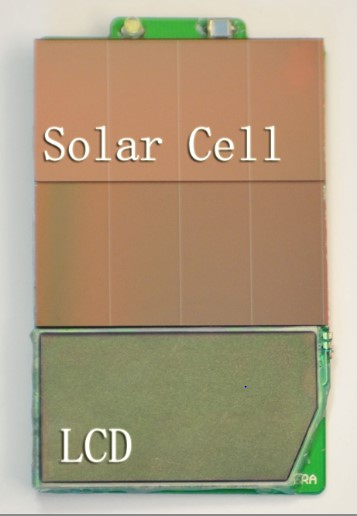
\includegraphics[width=0.45\columnwidth]{tag-front.jpg}
      } 
%      \hskip 1em
      \subfigure[\vitag Back]{
        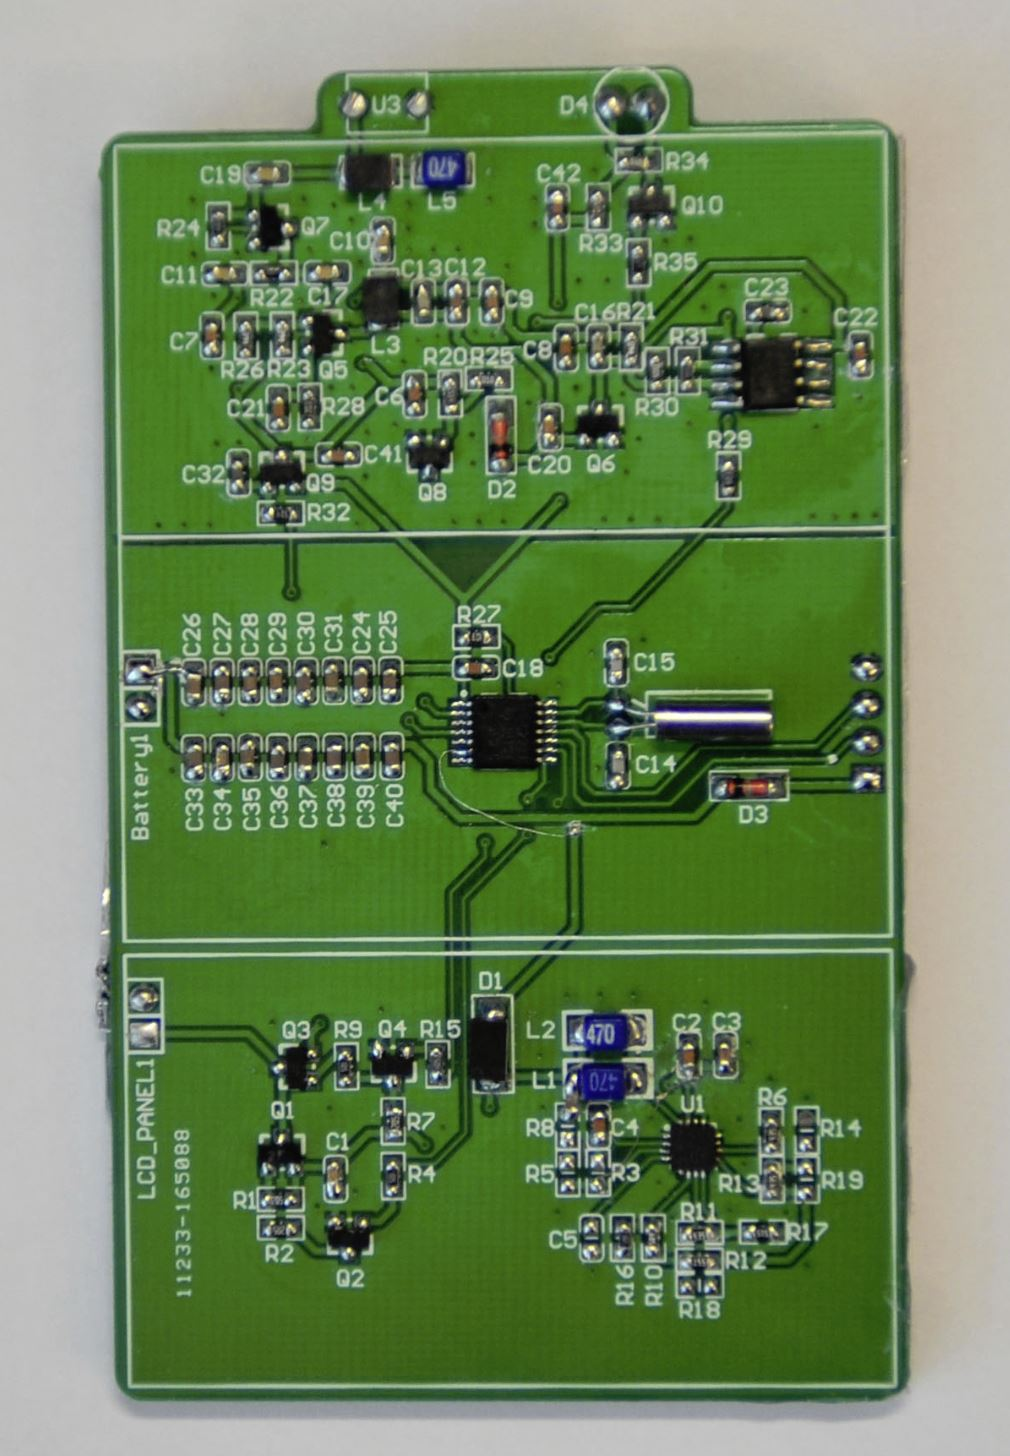
\includegraphics[width=0.45\columnwidth]{tag-back2.jpg}
      } 
%
      \subfigure[Lamp]{
        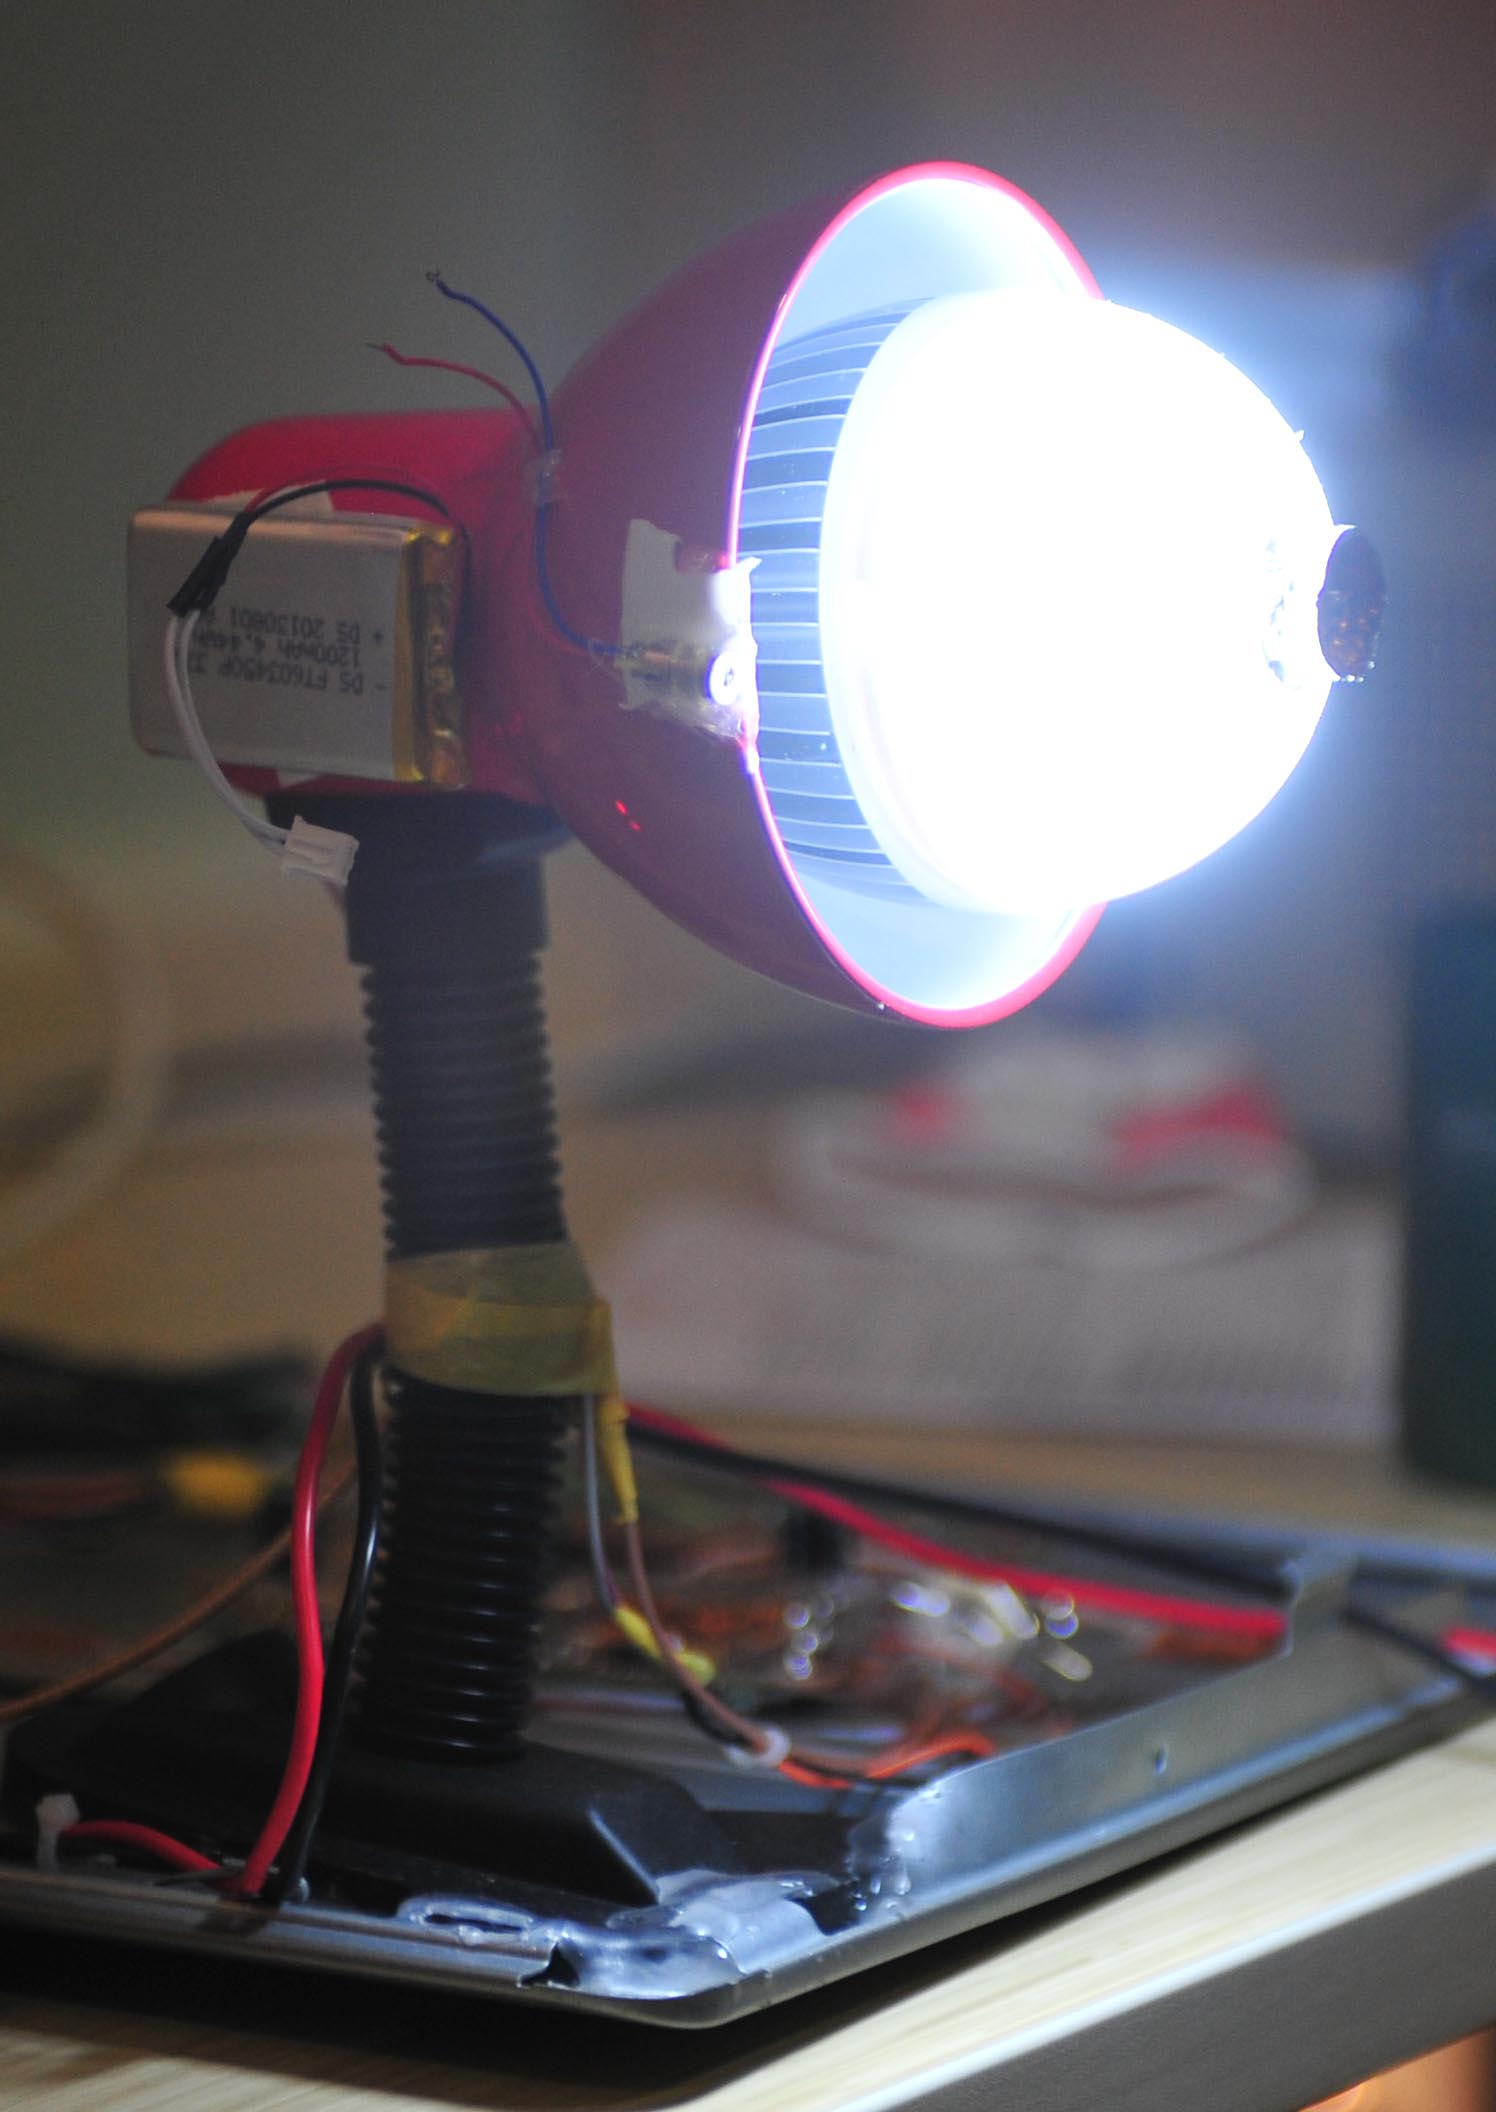
\includegraphics[width=0.47\columnwidth]{reader_lamp_2.jpg}
      } 
%      \hskip 1em
      \subfigure[Flashlight]{
        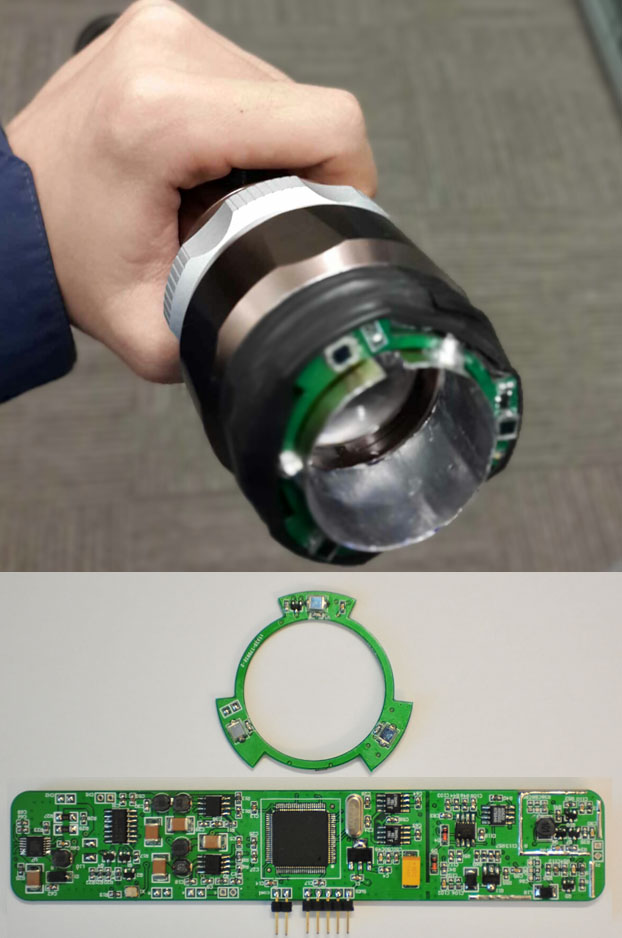
\includegraphics[width=0.44\columnwidth]{reader_torch.jpg}
      } 
\vspace{-1ex}      
\endminipage
\caption{Prototype.}
\label{fig:proto}
%\vspace{-1em}      
\end{figure}

\iffalse
\begin{figure}[!ht]
\centering
\minipage{.7\columnwidth}
      \subfigure[Lamp]{
        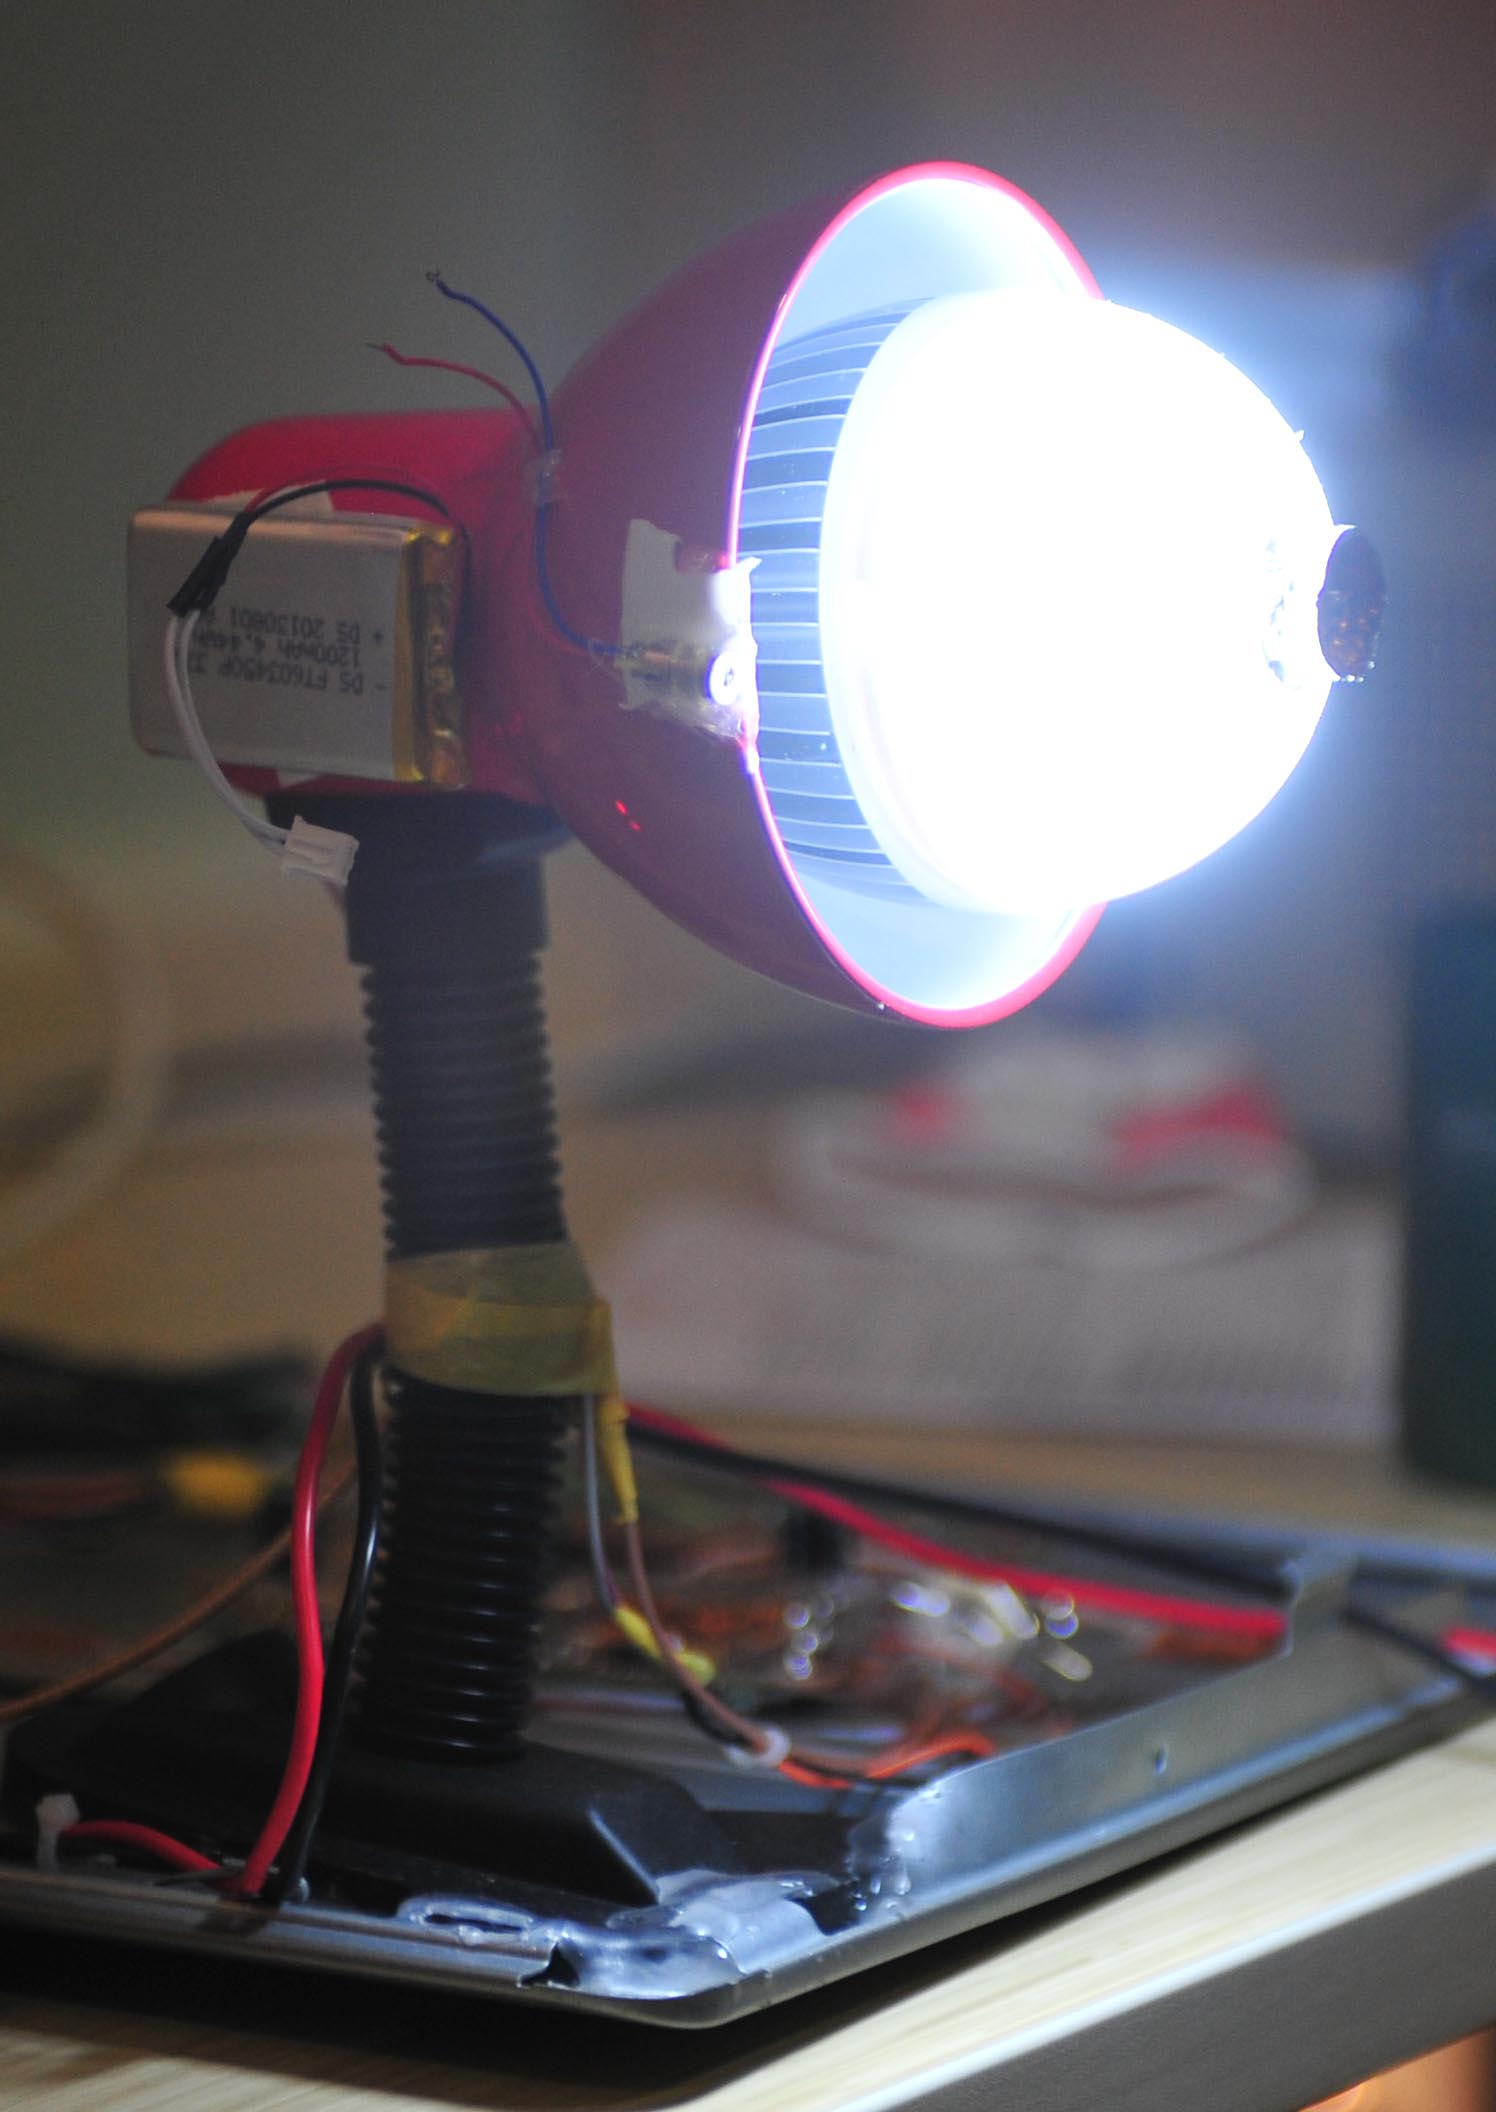
\includegraphics[width=0.47\columnwidth]{reader_lamp_2.jpg}
      } 
%      \hskip 1em
      \subfigure[Flashlight]{
        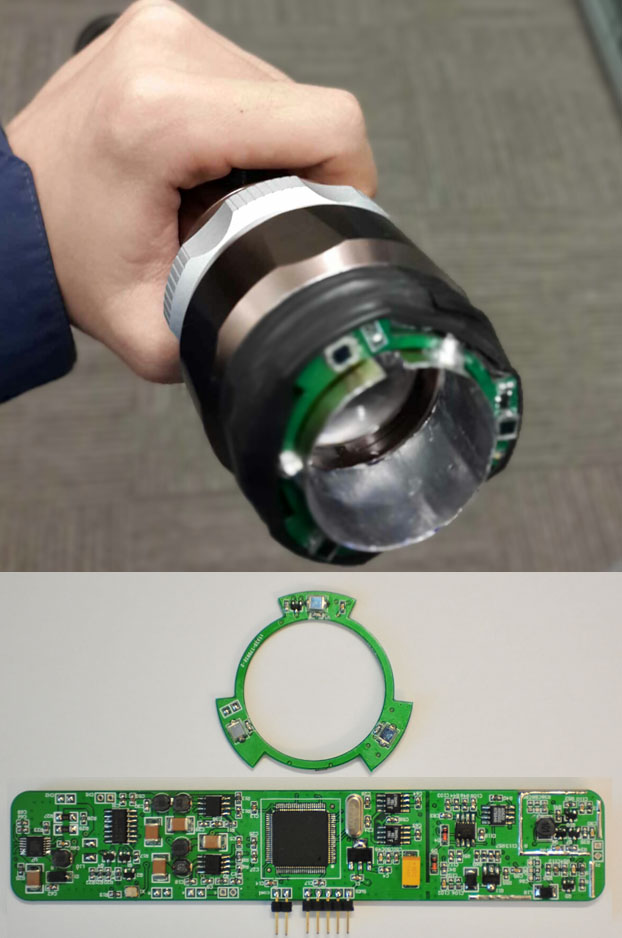
\includegraphics[width=0.44\columnwidth]{reader_torch.jpg}
      } 
\vspace{-1ex}      
\endminipage
\caption{Reader prototype.}
\label{fig:proto_reader}
%\vspace{-1em}      
\end{figure}
\fi

We use the schematics in \figref{fig:sysdiagram} in the implementation with printed circuit boards (PCBs) and off-the-shelf circuit components, which we summarize in Table~\ref{table:components}. The retro-reflector fabric we use is Scotchlite from 3M~\cite{rrsheet}. %We have implemented them as fully reconfigurable platforms, controlled by firmware executed on each individual microcontroller. 

\begin{table}[th]
\begin{center}
\small
\begin{tabular}{| l | l || l | l |}
\hline
\multicolumn{2}{ |c|| }{ \vitag\ } & \multicolumn{2}{ c| }{ \reader\ } \\ \hline\hline

Photodiode 		&  	BPW34 			& 	Photodiode 		&  	SFH213 			\\ \hline
MCU 			&	MSP430G	& 	MCU 			&	LPC4357		\\ \hline	
DC/DC 	&	BQ25504			& 	MOSFET 	&	IRF510			\\ \hline
Comparator		&	TLV2762			& 	Amplifier		&	\footnotesize{LM6172, AD620}			\\ \hline
Transistor		&	S9018 			& 	Transistor		&	\footnotesize{S9018, 2SC3357}			\\ \hline
LCD				&	SF110147 		& 	LED	Bulb			&	Apollo BR30 		\\ \hline
%Reflector 		&	\multicolumn{1}{ |c| } {3M Scotchlite} &  &  \\ \hline
\end{tabular}
\normalfont
%\vspace{-1em}      
\caption{Concrete models of electronic components used in \retro prototype}\label{table:components}
\end{center}
\end{table}

\begin{table}[h]
\begin{center}
\begin{tabular}{| l | l | l |}
\hline
Component\textbackslash Voltage 	& 	2.0V 						& 2.6V 								\\ \hline\hline

\multirow{2}{*}{Receiving Circuit} 	& $43.8\mu A$ 		& $48.4\mu A$ \\
									& ($87.6\mu W$) 	& ($125.8\mu W$) \\ \hline
 
\multirow{2}{*}{Transmitting Circuit} 	& $45.1\mu A$ 		& $36.7\mu A$ \\
									& ($90.2\mu W$) 	& ($95.4\mu W$) \\ \hline
									
\multirow{2}{*}{Total} 	& $91.9\mu A$ 		& $90.0\mu A$ \\
									& ($183.8\mu W$) 	& ($234.0\mu W$) \\ \hline									
\end{tabular}
%\vspace{-1em}
\caption{Overall and component-wise energy consumption of \vitag.}\label{table:energy}
\end{center}
\end{table}

The \reader\ is implemented in two forms. The first one is a lamp reader, which is modified from an $12W$ white LED lamp, as shown in \figref{fig:proto}(c). We put the light sensor inside the center of front surface of the lamp and isolate it with copper foil to reduce the leakage from the LED light. The second one is a flashlight reader, shown in \figref{fig:proto}(d). It uses a $3W$ LED as the transmitter. Three light sensors are used to improve the SNR. %The lamp reader is designed to work with large FOV but relatively short distance(about 2.5m, 50\degree), while the falshlight reader is designed to work with long distance with a narrower FOV (about 10.6m, 8.5\degree).


The energy consumption of \vitag is related to the voltage output of solar cell. We measure the overall and component-specific energy consumption for \vitag for two typical operating voltages, as shown in Table~\ref{table:energy}. The measurement shows that the \vitag prototype indeed achieves ultra-low power consumption. With such low power consumption, we are able to drive it by harvesting light energy using only small solar cells.

%\todo{If calculation supports that a single cell battery can last for years, then we can add some argument here saying that: In our prototype, two-thirds area is occupied by the solar cell. If smaller tags is desired, we can use cell battery. Our calculation indicate that a single xxx cell battery can last xxx long under xxx traffic.}

%MCU generated signal modulates the light and then we use a power MOSFET to implement an RF power amplifier. The amplified signal is sent to the bulb to be transmitted.

%The implementation of the \vitag\ receiver starts with a PIN photodiode as the light sensor. The captured signal is sent to a series of triode amplifiers and bandpass filters, after which the signal enters the high-gain demodulator.
%This demodulated signal is then sent to a comparator implemented using a TLV2762 operational amplifier, before the decoding process with an MSP430.

%In the \vitag\ transmitting phase, an SF110147 LCD is used, covering a retro-reflector fabric. For the energy reuse module, we use a diode to prevent the waste of the current and directs it to the recycling capacitor, and we use a BQ25504 to implement the DC-DC converter.

%The \reader\ receiver uses an SFH213 light sensor, parallel with an LC resonant circuit. It's followed by an impedance matching circuit and then the tuned differential amplifier, whose gain is controlled by the Cortex M4, aiming to decouple the RF interferences. Then we implement another two RF amplifiers using high frequency transistors. Sequentially, the active envelope detector is implemented using an LM6172 operational amplifier, along with 1N60 diodes. Finally, the signal passes through a baseband amplifier, arriving at the MCU ADC port.



%We notice that for a given lighting environment and a target \vitag size, there ought to be an optimal division between the area for solar cell and that for retro-reflector. 

%\p{liqul: we should have a dedicated section like "Trade-off of sizes" discussing how we partition the constrained board size into two retro-reflector and solar cell. The intuition is that we should not assign too much space to either side. There should be an optimal partitioning. Not sure if our current design is optimal.}

\iffalse
%\subsubsection{Solar Cell Size v.s. Communication Range}
\vskip 0.05in\noindent{\it Experiments.} We test how far the tag can be reached as we cover part of the solar cell.

\vskip 0.05in\noindent{\it Results.} Fig.~\ref{fig:solar} shows the solar cell area does not affect the communication range within a certain region. \hl{there is a threshold, above which succeed, below which fail}


\begin{figure}[tb!]
\centering
\includegraphics[width=0.7\columnwidth]{../evaluation/SolarCellSize_Range.eps}
\vskip -0.05in
\caption{\footnotesize{\bf Solar Cell Size V.S. Communication Range.} \todo{Need to explain the units of X-axis.}.}
\label{fig:solar}
\vskip -0.05in
\end{figure}

%\subsubsection{Reflector Size v.s. Communication Range}

\vskip 0.05in\noindent{\it Experiments.} We test how far the tag can be reached as we cover part of the retro-reflector.

\vskip 0.05in\noindent{\it Results.} Fig.~\ref{fig:retro} shows \hl{area covered proportional to range}

\begin{figure}[tb!]
\centering
\includegraphics[width=0.7\columnwidth]{../evaluation/ReflectorSize_Range.eps}
\vskip -0.05in
\caption{\footnotesize{\bf Retro-Reflector Size V.S. Communication Range.} \todo{Need to explain the units of X-axis. It's area, should be square cm.}.}
\label{fig:retro}
\vskip -0.05in
\end{figure}
\fi

\subsection{Potential Applications}
The low power duplex \retro system has many potential application scenarios. 

\paragraph{Home sensor bearer} Sensors such as motion, temperature, humidity and other sensors can be integrated with \vitag. Sensor readings can be streamed to a \reader-capable lighting LED. Such an application would benefit from the battery-free property of \vitag: deployment is extremely simple and sensors can remain untethered afterwards.   

\paragraph{Visible-light identification (VLID)} Taking visible light as the communicating media, VLID has many advantages over radio-frequency based identification systems, such as can achieve distant communication with battery free Tags, immune to electromagnetic interference, and more secure, thus it has the potential of replacing RFID in many scenarios such as in warehouses, storage and transportation systems.

\paragraph{Interactive road side traffic signs} The battery-free design of \vitag can be applied to road-side signs. Cars can communicate with them using LED headlights. Similarly, it can be used for automatic tollgate. 

\paragraph{NFC communication/payment} The use of visible light and the directional reflection property of the retro-reflector makes it a securer and faster means than other wireless NFC system.  The tag size can made smaller if only for short range communication. 

\section{Evaluation}
\label{sec:eva}

We evaluate \retro using our prototype implementation with a testbed shown in \figref{fig:setup}. The LED on the \reader is 12 Watt and the \vitag is of credit card size. As \reader is externally powered and the downlink signal are strong, (we achieved the designed data rate $10kbps$ on the downlink) we have thus focused on measuring the bottleneck uplink performance. The following system aspects are evaluated, namely, packet loss rate, response time, channel response and also the angle within which the uplink signal can be detected. The latter is to show the \retro system's ability against eavesdropping attacks. \fyi{Unless otherwise noted, evaluation about angle and response time is evaluated with the lamp reader.}

%unless otherwise noted

% in several aspects. As shown in Fig. \ref{fig:setup}, we have a pair of ViReader and ViTag residing in a horizontal 2D plane. First, we measure the packet loss rate (PLR) during reader-to-tag communication. Then, we evaluate the response time of our ViTag. Finally, we evaluate the system's ability against eavesdropping attacks. 

\begin{figure}[tb!]
\centering
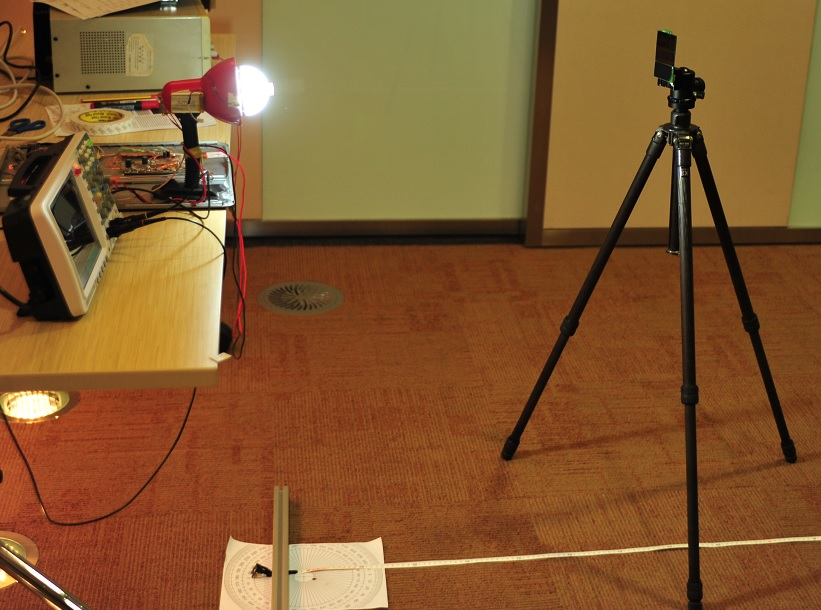
\includegraphics[width=0.7\columnwidth]{setup}
\vskip -0.05in
\caption{Evaluation testbed setup with a pair of ViReader and ViTag (For experiment with flash light reader, the lamp is replaced with flashlight reader).}
\label{fig:setup}
\vskip -0.05in
\end{figure}

%
%at various locations with different system settings. First we seek to validate it's point-to-point communication performance at varying data rates. Then we evaluate the security aspect of the system against a typical type of malicious behaviors, snifter.
%
%%\subsection{Evaluating the Communication Range}
%
%We evaluate the maximum communication distance between a \reader\ and a \vitag\ as a function of the LED illumination, solar cell size, retro-reflector size, tag orientation, angle of incidence at the reader and data rate. Maximum communication distance or range is defined as the longest distance at which the \vitag\ can respond to the \reader\. The \reader\ signals the successful receiving of a packet by a beep. We perform our experiments in three scenarios:
\paragraph{Testing Environments}
Being a VLC system specially designed for the indoor environments with lighting structure, we carried experiments in typical office environment, where the ambient light is maintained in a comfortable range around 300$lx$. The ViTag harvests energy not only from the \reader, but also from ambient light. On the other hand, the office environment comes with human movements and other disturbances that may affect communication. To give a sense of the environmental impact, we also test it in a dark chamber, as a baseline for comparison. In the dark chamber, the \reader LED is the sole light/energy source. 
%We note that the system performance is affected by the environment conditions. Therefore, we carry out evaluations in two representative environments: 
%\vskip 0.05in\noindent{\bf (1) Dark Chamber} Where the ViTag has the LED as the sole power source, a dark chamber also eliminates the environmental impact. This represents the controlled case which we use as the baseline. 
%\vskip 0.05in\noindent{\bf (2) Office ($\sim$300 Lux) } Offices are typical indoor places usually illuminated by artificial lighting systems. The ambient light is usually maintained within a comfort range around $300 Lux$. The ViTag harvests energy not only from the ViReader, but also from ambient light. However, the office environment comes with human movements and other disturbance that may affect communication.
                                                                                                                                                                                                                                                                                                                                                                                                                                                                                                                                                                                                                                                                                                                                                                                                                                                                                                                                                                                                                                                                                                                                                         
%\vskip 0.05in\noindent{\bf (3) Outdoor (day time)} Outdoor is another scenario where the ViTag actually gain energy from the sunlight \footnote{The outdoor night case is similar with the dark chamber which is thus not considered in our evaluations.}, which is different from artificial lighting. We perform our experiments on the sidewalk of a busy road. 
%\q{How would you do experiments for Night?}

\paragraph{Summary of Key Findings}
The key findings are highlighted as follows:
\begin{Itemize}
\item The experiments verify that we are able to get a \vitag\ to operate battery-free up to $2.4m$ away with lamp reader and $10.6m$ with flashlight reader (with package loss rate below $80\%$, or equivalent BER below $8.26\%$) and $0.5kbps$ data on the uplink. The system works for a wide range of \vitag orientations.
\item Reader-to-tag communication is resilient to eavesdropping. {\reader}s can only sense the ongoing communication in a visible range,  within a narrow the field of view of about $\pm 15\degree$.
\end{Itemize}

%\begin{figure*}[t]
%\minipage{0.32\textwidth}
%  \includegraphics[width=\textwidth]{../evaluation/PackageLostRate_Dark.eps}
%  \vspace{-2em}
%  \caption{Distance vs.\ packet loss rate in dark chamber and office room of 12W LED Lamp.}\label{fig:plr}
%\endminipage\hfill
%\minipage{0.32\textwidth}
%  \includegraphics[width=\textwidth]{../figures/angle_plr_100cm.eps}
%  \vspace{-2em}
%  \caption{Angle of incidence (irradiation) vs.\ packet loss rate.}\label{fig:readerAoI}
%\endminipage\hfill
%\minipage{0.32\textwidth}%
%  \includegraphics[width=\textwidth]{../figures/chargingtime_distance.eps}
%  \vspace{-2em}
%  \caption{Charging time vs.\ distance in dark chamber and office room.}\label{fig:charging_distance}
%\endminipage
%\end{figure*}


\subsection{Packet Loss Rate}\label{sec:plr}
%On the downlink, the transmitter is typically a powerful LED connected to the power line. Therefore, the bottleneck lies in the uplink. 
In this subsection, we focus on evaluating the packet loss rate (PLR) of the uplink tag-to-reader communication. For VLC, the received signal strength is mainly affected by three factors, i.e., the distance between ViTag and ViReader, the incidence angle, and the irradiation angle \cite{location3}.   

We first measure the impact of distance on PLR by varying the distance between ViReader and ViTag. We keep the ViReader perpendicular to the ViTag, i.e., $0\degree$ incidence or irradiation angles. To measure the PLR, the ViTag continuously sends packets for 20 minutes to ViReader with a constant rate. Each packet is consisted of $4 bytes$ ID data. We count the number of packets received successfully at ViReader. \figref{fig:plr} shows the resulting PLR versus distance. 

\begin{figure}[!ht]
\centering
\includegraphics[width=0.8\columnwidth]{../evaluation/PackageLostRate_Dark.eps}
\vskip -0.05in
\caption{Distance vs. PLR of 12W LED Lamp.}
\label{fig:plr}
\vskip -0.05in
\end{figure}

Figure ~\ref{fig:plr} shows that in a dark chamber, the PLR remains below $0.7\%$ in a distance up to $1.4m$. As the tag moves past $1.4m$, the PLR increases dramatically; Packets are barely received beyond $2.0m$. The drastic increase in PLR is because the energy obtained from the solar cell becomes insufficient in a long distance. In contrast, the PLR increases slower in the office environment thanks to the energy the ViTag harvests from the ambient light in addition to that from the ViReader. 

\begin{figure}[!ht]
\centering
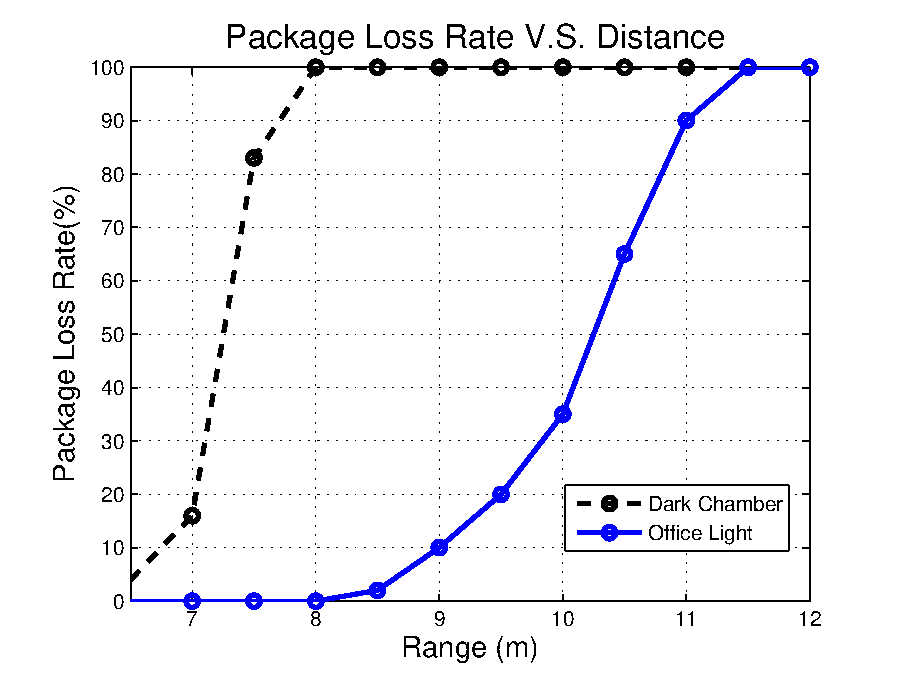
\includegraphics[width=0.8\columnwidth]{fig/PackageLostRate_flashlight.eps}
\vskip -0.05in
\caption{Distance vs. PLR of 3W flash light reader. X-axis starts from 6.5 meters}
\label{fig:plr_torch}
\vskip -0.05in
\end{figure}
Figure ~\ref{fig:plr_torch} presents the PLR as a function of the range for the 3W flash-light reader. The experiment shows that with the 3W flash-light reader, a much longer communication range can be reached. Specifically, in a dark chamber, instead of $1.4m$, the energy for receiving begins to drop significantly at $7.0m$, and nearly exhausts at $7.4m$. Under the situation with normal office lights, the system performs even better in terms of the communication range. The PLR remains at nearly 0 until the tag-reader distance reaches $8.5m$, and reaches $80\%$ at 10.6m. We can still receive package in a distance of $11.4m$.

%The dramatic increase in PLR is due to the threshold effect of the demodulator. We use a threshold during decoding the weak and noisy signal. In order to recover the drifting clock of the ViTag, we set a conservative threshold, and therefore lead to a sharp cut-off signal strength for successful decoding. 

\begin{figure}[!ht]
\centering
\includegraphics[width=0.8\columnwidth]{../figures/angle_plr_100cm.eps}
\vskip -0.05in
\caption{Angle of incidence (irradiation) vs.\ packet loss rate.}\label{fig:readerAoI}
\vskip -0.05in
\end{figure}

We then evaluate the PLR under different incidence or irradiation angles. Fix the distance between ViReader and the ViTag plane (the plane where the ViTag resides in 3D space), and move ViTag along the plane. In this setting, the incidence angle always equals the irradiation angle%\footnote{We note that these two angles are not identical in practice. However, our evaluation here represents the average case, and thus makes sense in reality.}. 
In our evaluation, we fixed the distance at $100$cm. The measured results are shown in \figref{fig:readerAoI}. We note that despite the seeming high PLR (\eg 80\%), for certain applications such as ID tag, we can still obtain the information after a few trials. This is similar to RFID systems. 



%\begin{figure}[tb!]
%\centering
%\includegraphics[width=0.45\columnwidth]{../figures/angle_plr_100cm.eps}
%\includegraphics[width=0.45\columnwidth]{../figures/angle_plr_200cm.eps}
%\vskip -0.05in
%\caption{\footnotesize{\bf Angle of incidence/irradiation at Reader V.S. PLR in a dark chamber and office room.} }
%\label{fig:readerAoI}
%\vskip -0.05in
%\end{figure}


%\paragraph{Maximum working range} We define the maximum communication range as the maximum distance between ViReader and ViTag such that ViReader is still able to decode the packet from ViTag. From Fig. \ref{fig:plr}, the maximum working range is thus 1.7 meters as discussed above.

\subsection{Response Time}\label{sec:bootstrap}
Response time accounts for the time from the ViReader issuing a query to receiving a response from the ViTag. Therefore, the response time consists of \textit{charging time}, downlink packet reception time, and uplink packet transmission time. Response time is a important metric for user experience. Generally, a response time below $100ms$ is thought to be negligible by human. In our system, due to the limitation of the LCD frequency, the uplink packet transmission time is slow, taking over $100ms$ to send a 32-bit ID. We envision faster LCD shutters in the future, and only focus on the charging time in the following.

\begin{figure}[!ht]
\centering
\includegraphics[width=0.8\columnwidth]{../figures/chargingtime_distance.eps}
\vskip -0.05in
\caption{Charging time vs.\ distance in dark chamber and office room.}\label{fig:charging_distance}
\vskip -0.05in
\end{figure}

If ViReader and ViTag are close enough, ViTag can quickly harvest enough energy to start conversation. Inversely, if the distance is long, ViTag needs a longer charging time before responding. We define the charging time as the time used to charge a \textbf{zero-initial-energy} ViTag. Charging time is affected by a number of factors like the solar cell size, ViTag energy consumption, and environment illumination level. %Among these, environment brightness has a significant impact on the charging time. For instance, in office area, the ViTag harvests energy from both the emitted light of ViReader and the existing indoor lighting system, thus reducing the charging time. 
As ViTag size is fixed, we only evaluate the impact from the environment illumination. 

First we evaluate the charging time as we vary the distance from $0.1m$ to $1.8m$, counting the time when the operation voltage raises from $10\%$ to $82.5\%$ (min operation voltage). The result is presented in Fig. \ref{fig:charging_distance}. We can see that, when the distance is small, the charging time in both cases are close. For instance, when the distance are $10$ or $20cm$, the charging time are around $50$ and $100ms$, respectively. The two curves begin to separate after around $0.6m$. The charging time in office environment grows slowly due to extra energy supply from the ambient light.


%\begin{figure}[tb!]
%\centering
%\includegraphics[width=0.7\columnwidth]{../figures/chargingtime_distance.eps} % {charging_time}
%\vskip -0.05in
%\caption{Charging time v.s. distance in a dark chamber and an office room. We show the raw measurements in markers and their polynomial fitting curves.}
%\label{fig:charging_distance}
%\vskip -0.05in
%\end{figure}
%

\begin{figure}[!ht]
\centering
\includegraphics[width=0.8\columnwidth] {../figures/angle_chargingtime.eps}
\vskip -0.05in
\caption{Charging time vs.\ incidence (irradiation) angles.}\label{fig:charging_angle}
\vskip -0.05in
\end{figure}

We note that the charging efficiency of the solar cell is also affected by the irradiation angle of the ViReader and also the incidence angle at the solar cell. For simplicity, we fix the distance between ViReader and the ViTag at $60$ and $120cm$, respectively, and observe charging time versus the incidence/irradiation angle shown in \figref{fig:charging_angle}. We indeed see increase in charging time with larger angles. However, the charging time grows slowly especially when the angle is small, e.g., below $30\degree$. This means the ViTag \fyi{tolerates flexible orientations} without experiencing serious performance degradation. In particular, we see much less sensitive reaction to the angles in office environment due to energy harvest from ambient light, which further highlights the benefit of using visible light as the power source.

%\begin{figure}[tb!]
%\centering
%\includegraphics[width=0.45\columnwidth]{../figures/chargingtime_angle_60cm.eps}
%\includegraphics[width=0.45\columnwidth]{../figures/chargingtime_angle_120cm.eps}
%\vskip -0.05in
%\caption{Charging time under different incidence/irradiation angles in a dark chamber and office room.} 
%\label{fig:charging_angle}
%\vskip -0.05in
%\end{figure}

In practice, ViTag can always harvest energy from ambient light (sunlight or artificial lighting systems) no matter whether a ViReader exists. Thus, the actual bootstrap can be instantaneous. This is a key difference from RFID/NFC tags where the operation energy can only be gained from a dedicated reader. 

\subsection{Channel Response}

\fyi{This subsection shows how energy of light signal attenuates against travelling distance along the visible channel. Here, the visible channel means the path along which the light signal traverses until it is received by the receiver of the reader, including the downlink, the retro-reflector, the LCD and the uplink.} For all backscatter systems, often times the energy of the signal received by the reader, which is reflected or backscattered by the tag, tends to be much weaker than the energy received by the tag, which poses a bottleneck for the system. %\fye{ According to the light reflection model of a standalone retro-reflector, the received energy attenuates proportionally to the square of the distance, which aligns with the theoretical model of the electromagnetic wave attenuation. Empirically, together with the lamp reader or the flashlight reader, however, the actual retro-reflector has a slightly diffusion angle, and the signal strength is affected by the non-linear auto-gain control (AGC) amplifier in the reader receiver. }
%
Thus, the energy efficiency is a crucial factor. To get an accurate picture of how energy diffuses as a function of the communication range, we measured the observed channel response for the lamp reader and flashlight reader. Fig.~\ref{fig:ChannelResponse} and Fig.~\ref{fig:ChannelResponse_flash} shows the energy calculated at the MCU, as the square of the output voltage. 
Note that the signal is captured and then measured by MCU, so it goes through Auto Gain Control(AGC) amplifier. 
From both figures, we see that when the tag is close to the LED, the signal is very strong and the AGC is effective. As a result, the portion of curves before AGC turned off goes down slowly. It actually almost completely suppresses the amplification when the signal is extremely strong (\ie, very close distance to the flashlight reader), as  shown in Fig.~\ref{fig:ChannelResponse_flash}. For both figures, after the point when AGC is turned off, \ie, always exerting maximum amplification, both curves attenuates at a rate square or cube of the distance.
\begin{figure}[!ht]
\centering
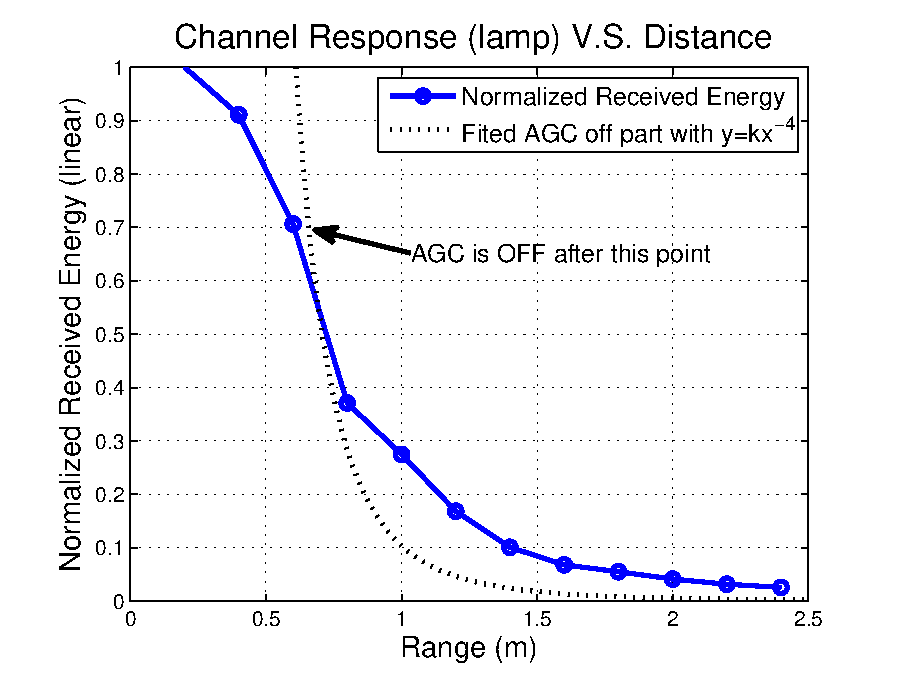
\includegraphics[width=0.77\columnwidth]{fig/ChannelResopnse_lamp.eps}
\vskip -0.05in
\caption{Channel responses of lamp reader}
\label{fig:ChannelResponse}
\vskip -0.05in
\end{figure}

\begin{figure}[!ht]
\centering
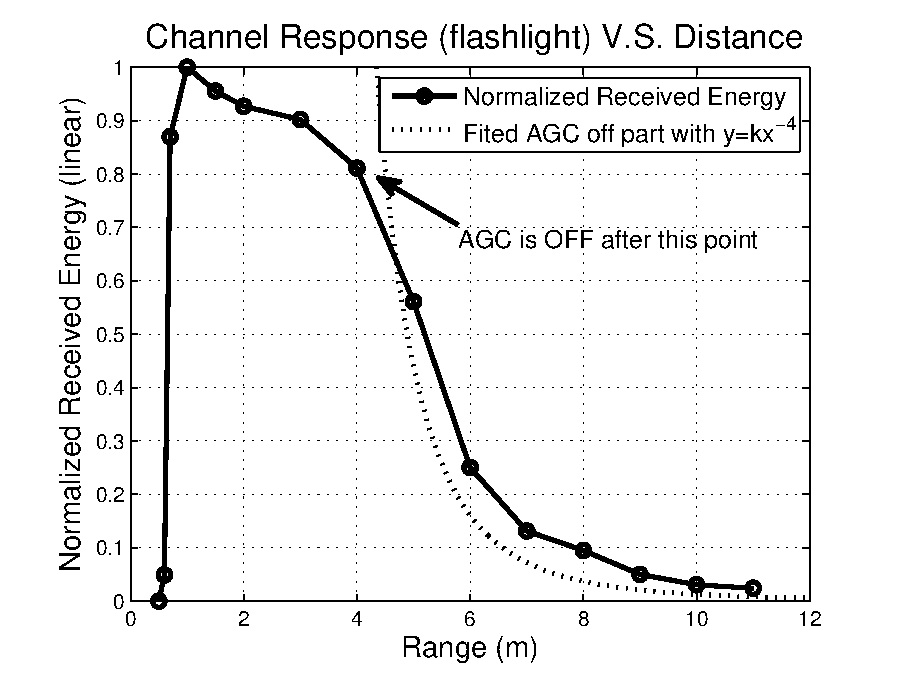
\includegraphics[width=0.77\columnwidth]{fig/ChannelResopnse_flashlight.eps}
\vskip -0.05in
\caption{Channel responses of flashlight reader}
\label{fig:ChannelResponse_flash}
\vskip -0.05in
\end{figure}


%

We note that, for a typical \textit{battery-free} backscatter system~\cite{abc1}, the wave front of the modulated backscattered signal received by reader from the tag attenuates proportionally to the power four of the communication range. A detailed formula can be found in paper~\cite{backscatterdeclay}.
%
As a comparison, we fit the part of the curve after AGC turns off to a negative quartic function, as the dotted line in Fig.~\ref{fig:ChannelResponse} and Fig.~\ref{fig:ChannelResponse_flash}. We can see that the negative quartic function attenuates much faster than our measurements. Thus, \retro achieves much better energy efficiency and can work at longer communication distance than typical battery-free backscatter systems for the same source emission power. This is perhaps due to the fact that \retro actually help concentrates lights from a scattering light source.%reflects light back along the same incoming direction with little scattering,}
% 


\subsection{Maximum Working Range}

We have so far evaluate both the PLR and energy harvesting. We then define the working range as the area within which the ViTag can harvest enough energy and talk with the ViReader with a chance above $20\%$, i.e., package loss rate is less than $80\%$. We measure the working range in office environment, and show the result in Fig. \ref{fig:ContinuesWorkingRange}. The working range in Fig. \ref{fig:ContinuesWorkingRange} is the area within the closed blue curve. With an upright orientation of the ViTag, the maximum working distance is up to $2.6m$. With ViReader perpendicular to the ViTag plane, the Field of View (FoV) is around $50\degree$. In our evaluation, we always make sure the same incidence angle and irradiation angle. Thus, the measured working range is conservative. In practice, if we orient the ViTag towards the ViReader, the FoV can be even larger. 

\begin{figure}[!ht]
\centering
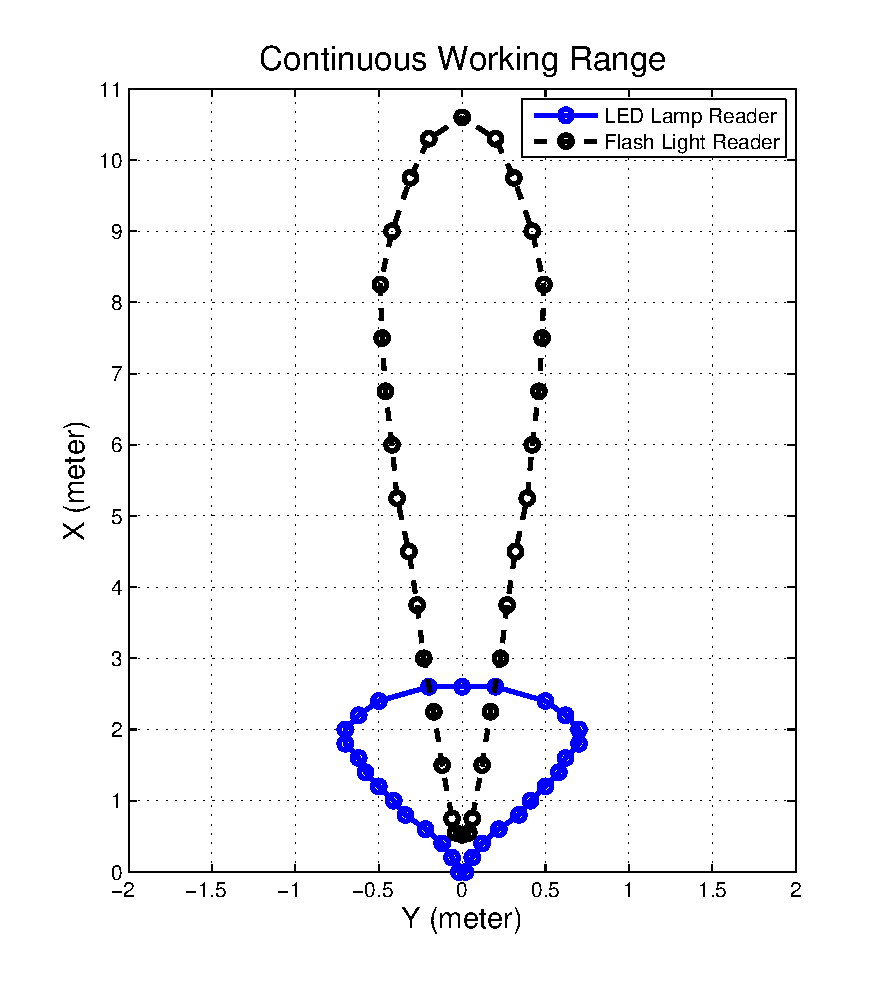
\includegraphics[width=0.7\columnwidth] {fig/ContinuesWorkingRange_flash.eps}
\vskip -0.05in
\caption{Working area measured in office environment. \fyi {Reader is located at (0,0).} }\label{fig:ContinuesWorkingRange}
\vskip -0.05in
\end{figure}

\fyi {As to flash-light reader, the max distance from the reader to the edge of the working area is 10.6m as shown in the figure. In our experiments, we can still receive packets at a maxim range of 11.3m. Note but, due to saturation, the flashlight reader can not work if the tag-reader distance is overly close, \eg., smaller than 0.5m, as show in \figref{fig:ContinuesWorkingRange}. This is due to the saturation of the sensors and amplification circuits. }

%\begin{figure}[tb!]
%\centering
%\includegraphics[width=0.8\columnwidth]{../figures/ContinuesWorkingRange.eps}
%\vskip -0.05in
%\caption{Working range measured in office environment.} 
%\label{fig:ContinuesWorkingRange}
%\vskip -0.05in
%\end{figure}

\subsection{Eavesdropping Range}\label{sec:secure}

Eavesdropping attacks in our system refer to a device secretly listening to the conversation between a ViTag and a ViReader. It is shown that eavesdropping is usually an early step of other attacks like man-in-the-middle attacks \cite{rfidsec1,rfidsec2}. One of the promising applications of \retro is using ViTag as a badge or payment card. Therefore, it is important that we protect the communication safety against eavesdropping attacks. 

\begin{figure}[!ht]
\centering
\includegraphics[width=0.7\columnwidth] {../figures/security_experiment_figure2.eps}
\vskip -0.05in
\caption{Signal detection radius of uplink. }\label{fig:security}
\vskip -0.05in
\end{figure}

A key feature of \retro compared with RFID/NFC is that the tag-to-reader communication is \textbf{directional}. Therefore, it is expected that a conversation from ViTag can only be detected within a narrow FoV. It is shown in \cite{eavesdrop2} that a sniffer can overhear NFC communication even over 1 meter away. In our evaluation, we place a ViReader and ViTag pair $0.6m$ apart from each other. The ViTag faces squarely to the ViReader, as shown in Fig. \ref{fig:security}. We use another reader as the attacker and measure the area where the attack can sniff the transmission from the ViTag. The area is plotted in Fig. \ref{fig:security}. 

%\begin{figure}[tb!]
%\centering
%\includegraphics[width=0.9\columnwidth]{../illustrations/security_experiment.eps}
%\vskip -0.05in
%\caption{\footnotesize{\bf Illumination v.s. Signal-Detectable Radius of Uplink.} The areas in both cases are spindle-shaped.}
%\label{fig:security}
%\vskip -0.05in
%\end{figure}

The signal can actually be detected quite far away as shown in Fig. \ref{fig:security}. As discussed in Fig. \ref{fig:plr}, 
The reason is that the retro-reflector is not perfect, it reflects the light back with a small diffusion angle. The intensity of light decays quickly with the angle. In our experiment, we use a sniffer that have {$100dBm$} gain(the same as our \reader), and the result shows the detectable area is nearly $2m$ in the back, excluding the shadow of the \reader.
%For This: the maximum range where the ViReader has a chance to receive packets from the ViTag is upto 2.6 meters. Therefore, the maximum signal-detectable distance from the ViReader is nearly 2 meters. 		
%Jinagtao: I'm wrong about that yesterday. Reader's Range have no relationship with the sniffer range. Because the angle is of much different between reader sensor and sniffer sensor when looking at the Tag. Thus the sniffer has less light intensity received.
However, the whole area resides within a small FoV of the ViTag, making it much easier for the user to discern the sniffer and can be blocked by a larger cover of \reader. Usually, the reader is fixed on the wall (e.g., a badge reader) which further reduces the signal-detectable area. 


%\q{If the maximum communication range is 2.6 meters, the round trip distance should be 2.6*2=5.2 meters. Then, the maximum signal-detectable distance is 5.2-0.6 = 4.6 meters. Is this what Jiangtao told me today??}

%\subsection{Evaluating \retro for Typical Applications}\label{sec:data_rate}
%In this section, we evaluate \retro in two typical applications. 
%
%The first application is using ViTag as a replacement of existing RFID/NFC cards, e.g., a badge. The use case is as follows. The user wears a credit card sized ViTag badge during work time. She needs to swipe her badge in front of a reader beside the door in order to get into a lab. Most existing badges are based on RFID which can only operate within a few centimeters from the reader. The range has to be short due to security considerations, which however make it less user friendly as the user has to explicitly do the badge swiping action. Basically, the communication between reader and RFID tag can easily be overheard in quite a large area even if the reader adopts a low transmission power \cite{guoliang's paper}. As shown in Section \ref{sec:secure}, the tag-to-reader transmission can only be heard within $\pm xx\degree$ ensuring the security even the distance is far. Therefore, with our ViTag badge, the user can actually remotely and automatically swipe the badge without explicit actions. 
%
%For the ViTag badge application, the key metric is the response time, i.e., how long the user needs to wait before the ViReader successfully decode the ViTag's ID. The waiting time depends on both the charging time and the BER. Generally, the longer the distance and the more slant the incidence/irradiation angles, the longer the waiting time. 

%\vskip 0.05in\noindent{\it Experiments.} We evaluate the communication range the system can achieve at a set of downlink and uplink data rates. The downlink rates tested include \hl{5kbps, 2kbps and 1kbps}, and the uplink rates tested include \hl{0.125kbps, 0.5kbps, 1kbps}. The downlink is set to \hl{5kbps} when evaluating the uplink, and the uplink is set to \hl{0.125kbps} when evaluating the downlink.
%
%\vskip 0.05in\noindent{\it Results.} Fig.~\ref{fig:datarate} (a) shows \hl{Shannon theorem} \hl{uplink data rate can be improved by using smaller voltage span for the LCD, which is enforced in the firmware instead of making modifications to the circuit}. Fig.~\ref{fig:datarate} (b) shows ...
%
%
%
%
%\begin{figure*}[!t]
%\vskip -0.1in
%\centering
%{\footnotesize
%\begin{tabular}{cc}
%\epsfig{file=../evaluation/DownRate_Range.eps, width=0.4\columnwidth} & \epsfig{file=../evaluation/UpRate_Range.eps, width=0.4\columnwidth}\\
%{(a) Evaluating Downlink}  & {(b) Evaluating Uplink}\\
%\end{tabular}
%}
%%\vskip -0.1in
%\caption{\footnotesize{\bf Data Rate V.S. Communication Range.} Blah Blah.}
%\label{fig:datarate}
%\vspace{-1em}
%\end{figure*}




%\subsubsection{Illumination v.s. BER}
%
%\begin{figure}[tb!]
%\centering
%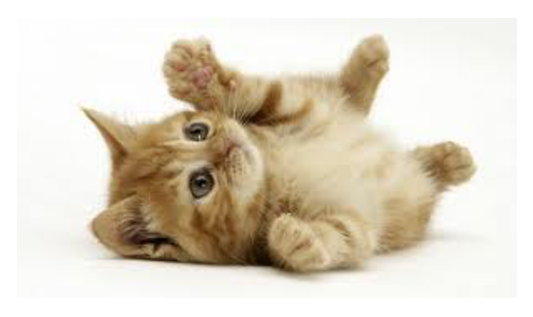
\includegraphics[width=0.7\columnwidth]{../figures/placeholder.eps}
%\vskip -0.05in
%\caption{\footnotesize{\bf Illumination v.s. BER.} blah blah.}
%\label{fig:ber1}
%\vskip -0.05in
%\end{figure}
%
%\subsubsection{Distance v.s. BER}
%
%\begin{figure}[tb!]
%\centering
%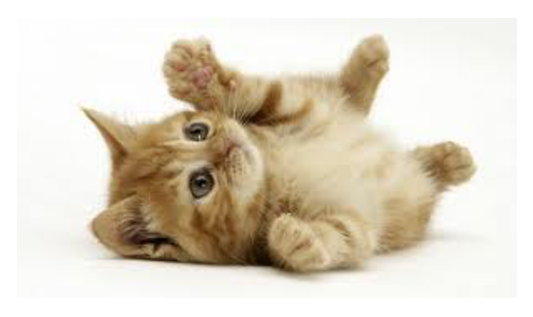
\includegraphics[width=0.7\columnwidth]{../figures/placeholder.eps}
%\vskip -0.05in
%\caption{\footnotesize{\bf Distance v.s. BER.} blah blah.}
%\label{fig:ber2}
%\vskip -0.05in
%\end{figure}

% \subsubsection{Retro-reflector Scattering}
% Due to surface defects, for example, not perfectly perpendicular micro-mirrors in the cubes, retro-reflectors render the reflected light scattered. We use \qm{a laser} that emits a nearly collimated beam to measure the scattering angle of the retro-reflector, with comparison to mirrors. Theoretically, suppose the mirror is not perfect, with an error angle $\Delta\theta$ that captures its surface defects. Suppose the retro-reflector has the same error angle that captures its surface defects on each of the three mirrors within a cube. 
% \q{What's this set of experiments aim at?}
% %\subsubsection{Illumination v.s. Charging time}


% \q{What kind of conclusion do we get from these experiments?}





% \subsubsection{Illumination v.s. Signal-Detectable Distance from the Tag}




% \begin{figure}[tb!]
% \centering
% 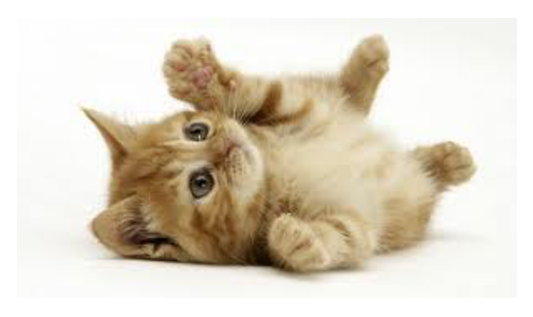
\includegraphics[width=0.7\columnwidth]{../figures/placeholder.eps}
% \vskip -0.05in
% \caption{\footnotesize{\bf Illumination v.s. Signal-Detectable Distance from the Tag.} blah blah.}
% \label{fig:security2}
% \vskip -0.05in
% \end{figure}



% \subsection{Evaluating Concurrent Transmissions}

% \subsubsection{\# of \vitag\/s Supported v.s. Communication Range}
% \hl{need another tag}
% \subsubsection{\# of \reader\/s Supported v.s. Communication Range}
% \hl{need another tag}




\section{conclusion}
In this paper, we have presented a bi-directional VLC system called \retro that consists of a modified LED and a tag device. The tag can run battery-free by harvesting light energy with solar cells. The \vitag\ transmits by reflecting and modulating incoming light back to the LED using a retro-reflector and an LCD modulator. The system overcomes the power consumption challenge on the \vitag and interferences and clock offsets on the LED end, achieving $10kbps$ downlink rate and $0.5kbps$ uplink rate over a distance up to $2.4m$. The system also shows security advantages, preventing readers nearby from overhearing uplink data. We believe \retro have wide application scenarios.  

% make the bibliography compact: use only in desperate situations
\let\oldthebibliography=\thebibliography
\let\endoldthebibliography=\endthebibliography
\renewenvironment{thebibliography}[1]{%
    \begin{oldthebibliography}{#1}%
      \setlength{\parskip}{0ex}%
      \setlength{\itemsep}{0ex}%
}%
{%
\end{oldthebibliography}%
}
{
\small
\bibliographystyle{abbrv}
\bibliography{ourbib}
\begin{appendix}
\section*{Appendix}
\label{sec:app}
\noindent{\bf Proof of Lemma~\ref{lem:lemma1}} 
%Assume the estimated end of the preamble (the beginning of the payload) is $\hat{t_0}$, and the actual beginning of the payload is $t_0$. 
Assume the first estimated preamble bit is at $\hat{t_0}$, and its actual time $t_0$. 
Denote $s[n]$ as the central time of a three bit sequence on \readerrx, and $t[n]$ as the central time of a three bit sequence on \tagtx, where $t[n+1]-t[n]$ is the time period of one bit ($n:0, 1, ..., +\infty$). We have
\begin{align*}
t[n]=t_0+k\cdot s[n]
\end{align*}
where $k\cdot s[n]$ is a mapping from the \readerrx to the actual bit boundaries, which we suppose is linear on the small bit-period time scale. The problem is then, given $\hat{t_0}$, $s$ and $t[i]$,
%\footnote{We already have an accurate $t[i]$ as we perform the wave form matching and time recovery algorithm introduced in~\ref{subsubsec:clockoffset}}, 
estimate the next actual bit boundary $t[i+1]$. Our method is to approach the above equation by drawing a line that connects $(s[i], t[i])$ and $(0, \hat{t_0})$ as the following
\begin{align*}
\hat t[i+1]=\hat{t_0}+\frac{t[i]-\hat{t_0}}{s[i]}s[i+1]
\end{align*}
Therefore
\begin{align*}
error_{time}=&\lim_{i\to\infty}\hat t[i+1]-t[i+1]\\
=&\lim_{i\to\infty}\hat{t_0}+\frac{(t_0+k\cdot s[i])-\hat{t_0}}{s[i]}s[i+1]\\
& \qquad -(t_0+k\cdot s[i+1])\\
=&\lim_{i\to\infty}(\hat{t_0}-t_0)(1-\frac{s[i+1]}{s[i]})=0
\end{align*}
The result highlights that the deviation of the bit boundary estimate will not propagate, and will converge to zero for infinitely long packets.

\iffalse
\noindent{\bf B. Proof of Lemma~\ref{lem:lemma2}} 
Our goal is to prove that using the combination of an LCD and a retro-reflector as a passive emitter is more energy-efficient than using an LED as an active emitter when both systems have the same \reader\ whose LED has a power $P_0$, bit rate $1/\Delta t$, \reader-to-\vitag\ distance $r$, energy used for transmitting per bit $E_{tx}$ and receiving per bit $E_{rx}$, and noise power. We compare the SNRs at \reader\ receiver for the two methods. Further, since the noise power in the two scenarios are the same, we need only compare the quantities of the signal energy per bit $E_{s1}$ and $E_{s2}$. The system with the larger one has a better energy efficiency.

First, for the LCD tag with a retro-reflector, all the energy it transmits is received by the \reader\ receiver, assuming the LED on \reader\ is at the same location with the light sensor. Also, the signal \vitag\ receives is modulated and bounced back. Therefore
\begin{align}
E_{s1}=\eta_1\frac{P_0\Delta t}{4\pi r^2}\Delta S_{tag}
\end{align}
where $\eta_1$ accounts for the energy dissipation caused by the absorption of the retro-reflector and the direct reflection of the LCD, and $S_{tag}$ denotes the equivalent reflective area on the tag.

Second, for the LED tag that actively transmits, in a bit period, we have
\begin{align}
E_{s2}=\eta_2\frac{E_{tx}}{4\pi r^2}\Delta S_{reader}
\end{align} 
where $\eta_1$ is the efficiency of the LED tag hardware, and $S_{reader}$ denotes the light sensor area on the reader.

Finally, as we have assumed that the power supplies for both the systems are identical, and for the LCD tag, $E_{tx}=kCV^2$, where $k$ captures the efficiency of the energy reuse module and $CV^2$ denotes the energy cost per LCD capacitor period that corresponds to transmitting one bit, we have
\begin{align}
\frac{E_{s1}}{E_{s2}}=\frac{\eta_1 P_0\Delta t\Delta S_{tag}}{\eta_2 kCV^2\Delta S_{reader}}
\end{align}

Typically, $V=5V$, $C=2000pF$, $k\approx 0.4$, $\eta_1\approx 10^{-2}$, $\eta_2\approx 0.8$, $P_0=8W$, $\Delta S_{reader}=2\times 10^{-5}$ and $\Delta S_{tag}=10^{-3}$. So $\frac{E_{s1}}{E_{s2}}=10^9 \left|\Delta t\right|$. This result shows that if the data rate $1/\Delta t$ is smaller than $10^9bps(=1Gbps)$, then an LCD tag always enables higher energy per bit at the \reader\ receiver than an LED tag. In typical indoor settings, LEDs are primarily used for lighting, the upper bound of whose flickering rate is orders of magnitude smaller than $1GHz$; That is to say, our method is always more energy-efficient than the alternative LED tag.
\fi
\end{appendix}
}
\small
\end{sloppypar}
\end{document}


